\documentclass[10pt,letterpaper]{article}
\usepackage[top=0.85in,left=1.0in,right=1.0in,footskip=0.75in]{geometry}

% Use adjustwidth environment to exceed column width (see example table in text)
\usepackage{changepage}

% Use Unicode characters when possible
\usepackage[utf8]{inputenc}

% textcomp package and marvosym package for additional characters
\usepackage{textcomp,marvosym}

% fixltx2e package for \textsubscript
\usepackage{fixltx2e}

% amsmath and amssymb packages, useful for mathematical formulas and symbols
\usepackage{amsmath,amssymb}

% cite package, to clean up citations in the main text. Do not remove.
\usepackage{cite}

% Use nameref to cite supporting information files (see Supporting Information section for more info)
\usepackage{nameref,hyperref}

\usepackage{amsthm}

% line numbers
\usepackage[right]{lineno}

% ligatures disabled
\usepackage{microtype}
\DisableLigatures[f]{encoding = *, family = * }

% rotating package for sideways tables
\usepackage{rotating}

% adding colored text for Noah's complaints.
\usepackage{color}

% for the beautiful checkmarks
\usepackage{pifont}

% Remove comment for double spacing
%\usepackage{setspace} 
%\doublespacing

% Text layout
\raggedright
\setlength{\parindent}{0.5cm}
\textwidth 6.25in 
\textheight 8.75in

% Bold the 'Figure #' in the caption and separate it from the title/caption with a period
% Captions will be left justified
\usepackage[aboveskip=1pt,labelfont=bf,labelsep=period,justification=raggedright,singlelinecheck=off]{caption}

% Bib stuff
\usepackage{natbib}

% Remove brackets from numbering in List of References
\makeatletter
\renewcommand{\@biblabel}[1]{\quad#1.}
\makeatother

\newtheorem{theorem}{Theorem}
\newtheorem{corollary}{Corollary}
\newtheorem{lemma}{Lemma}
\newtheorem{definition}{Definition}
\newtheorem{condition}{Condition}

\DeclareMathOperator*{\argmin}{arg\,min}

\newcommand*{\vertbar}{\rule[-1ex]{0.5pt}{2.5ex}}

% Leave date blank
\date{}

% Header and Footer with logo
\usepackage{lastpage,fancyhdr,graphicx}
\usepackage{epstopdf}
\pagestyle{myheadings}
\pagestyle{fancy}
\fancyhf{}

\rfoot{\thepage/\pageref{LastPage}}
\renewcommand{\footrule}{\hrule height 2pt \vspace{2mm}}
\fancyheadoffset[L]{2.25in}
\fancyfootoffset[L]{2.25in}
\lfoot{\sf PLOS}

%% END MACROS SECTION
\begin{document}
\vspace*{0.35in}

\begin{flushleft}
{\Large
\textbf\newline{Descent-based joint optimization}
}
\newline
\\
Jean Feng and Noah Simon
\\

\end{flushleft}
\section*{Abstract}
Tuning regularization parameters in regression problems allows one to control model complexity and induce desired structure. The current method of searching over a $k$-dimensional grid of parameter values is computationally intractable for $k>2$. We propose tuning the penalty parameters by treating it as a continuous optimization problem and updating the parameter values using a descent-based approach. Compared to performing cross validation over a grid, our method is significantly more efficient while achieving the same performance. This descent-based approach enables us to test regularizations with many penalty parameters, through which we discover new regularization methods with superior accuracy. Our experiments are performed on simulated and real data.

\section{Introduction}

Consider the usual regression framework with $p$ features, $x_{i1},\ldots,x_{ip}$ and a response $y_i$ measured on each of $i=1,\ldots,n$ observations. Let $X$ denote the $n \times p$ design matrix and $y$ the response vector. Our goal here is to characterize the conditional relationship between $y$ and $X$. In simple low-dimensional problems this is often done by constructing an $f$ (in some pre-specified class $\mathcal{F}$) that minimizes a measure of discrepancy between $y$ and $f(X)$ (generally quantified with some pre-specified loss, $L$). Often $\mathcal{F}$ will endow $f$ with some simple form (eg. a linear function). For ill-posed or high-dimensional problems ($p \gg n$), there can often be an infinite number of solutions that minimize the loss function $L$ but have high generalization error. A common solution is to use regularization, or penalization, to select models with desirable properties, such as smoothness and sparsity.

In recent years, there has been much interest in combining regularization methods to produce models with multiple desired characteristics. Examples include the elastic net \citep{zou2003regression}, which combines the lasso and ridge penalties, and the sparse group lasso \citep{simon2013sparse}, which combines the group lasso and lasso penalties. The general form of these regression problems is:

\begin{equation} \label {eq:basic}
\hat f(\lambda_1, ..., \lambda_J) = \argmin_{f\in\mathcal{F}} L(\boldsymbol{y}, f (\boldsymbol{X})) + \sum\limits_{i=1}^J \lambda_i P_i(f)
\end{equation}
where $\{P_i\}_{i=1, ..., J}$ are the penalty functions, and $\{\lambda_i\}_{i=1, ..., J}$ are the regularization parameters.

Regularization parameters control the degree of various facets of model complexity (e.g. amount of sparsity or smoothness). Often, the goal is to set the parameters to minimize the fitted model's generalization error. One usually estimates this using a training/validation approach (or cross-validation). There one fits a model on a training set $(X_T, \boldsymbol y_T)$ and measures the model's error on a validation set $(X_V, \boldsymbol y_V)$. The goal then is to choose penalty parameters, $\lambda_1, \ldots, \lambda_J$, that minimize the validation error, as formulated in the following optimization problem:
\begin{equation}
\begin{array}{c}
\min_{\boldsymbol{\lambda} \in \Lambda} L(\boldsymbol{y}_V, \hat f (\boldsymbol{X}_V | \boldsymbol{\lambda})) \\
\text{where } \hat f(\cdot | \boldsymbol{\lambda}) = \argmin_{f\in\mathcal{F}} L(\boldsymbol{y}_T, f (\boldsymbol{X}_T)) + \sum\limits_{i=1}^J \lambda_i P_i(f)
\end{array}
\label{jointopt}
\end{equation}
Here $\Lambda$ is some set that $\boldsymbol{\lambda}$ are known to be in (possibly just $\mathbb{R}^{n+}$).

The simplest approach to solving \eqref{jointopt} is brute force: one fits models over a grid of parameter values and selects the model with the lowest validation error. As long as the grid is large and fine enough, this method of ``grid search" will find a solution close to the global optimum. This approach is the current standard for choosing penalty parameters via training/validation. Unfortunately, it is computationally intractable in cases with more than two parameters. Many variants of grid search have been proposed to increase efficiency, but their runtimes are all exponential in the number of parameters.

In this paper, we propose leveraging the tools of optimization to solve \eqref{jointopt} over the penalty parameter space. We give a gradient descent algorithm for the penalty parameters (to minimize validation error). In contrast to an exhaustive ``grid search'', this ``descent-based'' optimization makes use of the smoothness of our validation-error surface. \eqref{jointopt} is generally not convex and thus we may not find the global minimum with a simple descent-based approach. However, in practice we find that simple descent gives competitive solutions.

In simulation studies we show that our descent-based optimization produces solutions with the same validation error as those from grid search. In addition, we find that our approach is highly efficient and can solve regressions with hundreds of penalty parameters. Finally, we use this method to analyze regularization methods that were previously computationally intractable. Through this, we discover that a variant of sparse group lasso with many more penalty parameters can significantly decrease error and produce more meaningful models.

\citet{lorbert2010descent} presented some related work on this topic. They solved linear regression problems by updating regression coefficients and regularization parameters using cyclical coordinate gradient descent. We take a more general approach that allows us to apply this descent-based optimization to a wide array of problems. In particular this paper focuses on three examples that demonstrate the wide applicability of our method: elastic net, sparse group lasso, and additive partial linear models.

In Section 2, we describe descent-based optimization in detail and present an algorithm for solving it in example regressions. In Section 3, we show that our method achieves validation errors as low as those achieved by grid search. In Section 4, we explore variants of the example regression problems that have many more regularization parameters and demonstrate that solving \eqref{jointopt} is still computationally tractable. Finally, we present results on data predicting colitis status from gene expression in Section 5.

\section{Descent-based Joint Optimization}
\subsection{Definition}
In this manuscript we will restrict ourselves to classes, $\mathcal{F}$, which, for a fixed $n$, are finite dimensional; ie. can be rewritten as $\mathcal{F} = \left\{f_{\theta}\middle|\theta\in\Theta\right\}$ for some finite dimensional $\Theta$. This is not a large restriction: The class of linear functions functions meets this requirement; as does any class of finite dimensional parametric functions. Even non-parametric methods generally either use a growing basis expansion (eg. Polynomial regression, smoothing-splines, wavelet-based-regression, locally-adaptive regression splines \citep{tsybakov2008introduction}, \citep{wahba1981spline}, \citep{donoho1994ideal}, \citep{mammen1997locally}), or only evaluate the function at the observed data-points (eg. trend filtering, fused lasso, \citep{kim2009ell_1}, \citep{tibshirani2005sparsity}). In these non-parametric problems, for any fixed $n$, $\mathcal{F}$ is representable as a finite dimensional class.
We can therefore rewrite \eqref{eq:basic} in the following form:

\begin{equation}\label{eq:train_disc}
\argmin_{\theta \in \Theta} L(\boldsymbol{y}, f_\theta(\boldsymbol{X})) + \sum\limits_{i=1}^J \lambda_i P_i(\theta)
\end{equation}

Suppose that we use a training/validation split to select penalty parameters $\boldsymbol{\lambda} = (\lambda_1, ..., \lambda_J)^\top$. Let the data be partitioned into a training set $(\boldsymbol{y}_T , \boldsymbol{X}_T)$ and validation set $(\boldsymbol{y}_V, \boldsymbol{X}_V)$. We can rewrite the joint optimization problem \eqref{jointopt} over this finite-dimensional class as:
\begin{equation}
\begin{array}{c}
\argmin_{\boldsymbol{\lambda} \in \mathbb{R}^k} L(\boldsymbol{y}_V, f_{\hat{\theta}(\boldsymbol{\lambda})}(\boldsymbol{X}_V)) \\
\text{where } {\hat{\theta}(\boldsymbol{\lambda})} = \argmin_{\theta \in \Theta} L(\boldsymbol{y}_T, f_\theta (\boldsymbol{X}_T)) + \sum\limits_{i=1}^J \lambda_i P_i(\theta)
\end{array}
\label{jointopt2}
\end{equation}
For the remained of the manuscript we will assume that \eqref{eq:train_disc} is strictly convex in $\theta$. This ensures that there is a unique solution to \eqref{eq:train_disc} which perturbs continuously in $\boldsymbol{\lambda}$.

\eqref{jointopt2} is the explicit, though often unstated, criterion that training/validation methods attempt to minimize to choose penalty parameters. The current standard is to minimize this using an exhaustive grid-search. Grid-based methods solve the joint optimization problem by fitting models over a $J$-dimensional grid $G$ in the penalty parameter space --- the computational runtime of grid-based methods grows exponentially with the number of parameters. While the approach is simple and powerful for a single penalty parameter, optimizing even moderate dimensional functions (3+) via exhaustive grid search is inefficient (and quickly becomes completely intractable).  In addition, \eqref{jointopt2} is generally a continuous, piecewise-smooth problem. Using an exhaustive search ignores information available from the smoothness of the surface. 

We propose leveraging the tools of smooth optimization to solve \eqref{jointopt2}. In particular we discuss iterative methods, based on walking in a descent direction until convergence to a local minimum. In the simple case where the criterion is differentiable with respect to the penalty parameters, it is straightforward to use gradient descent or some variant thereof. We show that, with some slight tweaks, gradient descent can be applied in situations where the penalty is only differentiable when restricted to directions involving a differentiable set.

Figure \ref{fig:compare} illustrates the differences between the two approaches. Grid-based method fits a model at every grid point, even though many of these grid points are not close to the global or local minima. We can save significant computational time if we avoid those points unlikely to yield good models. By incorporating information about the shape of the local neighborhood, descent-based methods choose an intelligent descent direction and explore the space more efficiently. 

\begin{figure}
\begin{center}
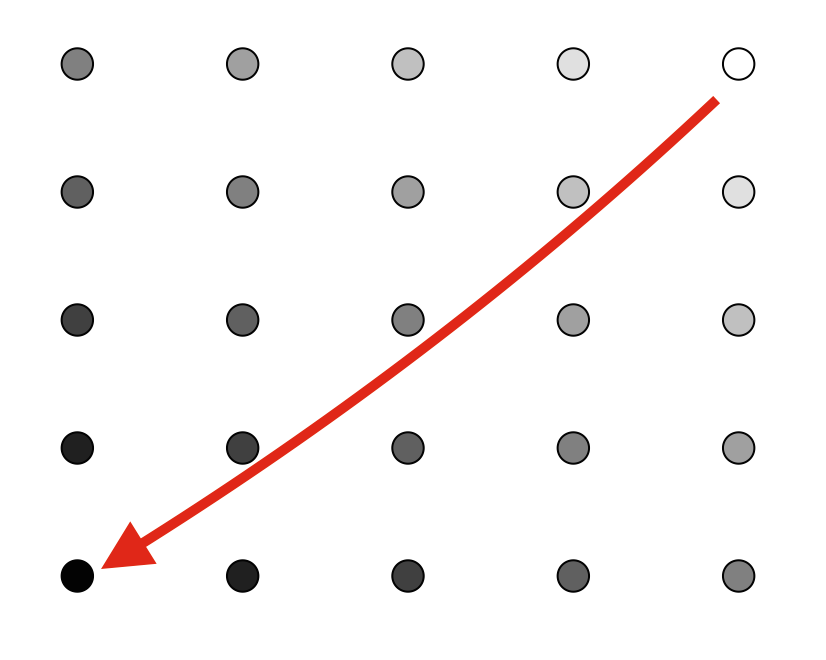
\includegraphics[height=40mm]{grid_search_vs_descent.png}
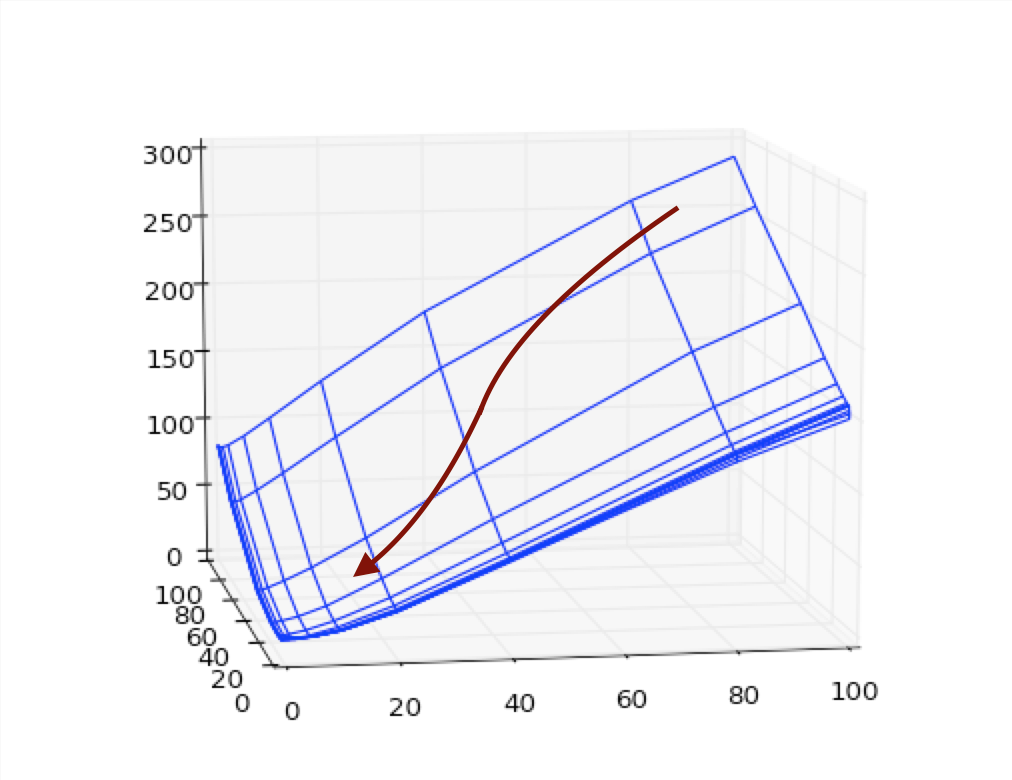
\includegraphics[height=60mm]{surface_in_regularization_parameters.png}
\end{center}
\caption{Left: darker points mean lower validation loss. Descent-based optimization descends in the most direct path towards the point producing the lowest validation loss. Right: The 3D version. We can tune regularization parameters using a grid search... or just descend opposite of the gradient.}
\label{fig:compare}
\end{figure}

Of course, the joint optimization problem is non-convex and therefore our method provides no guarantees, though, in practice, we have seen strong empirical performance. The major benefit of using our method is that it opens up the possibility of using regularization methods that combine many penalty terms.

To ease exposition, we will assume throughout the remainder of the manuscript that $L \Big( \boldsymbol{y}_V, f_{\theta}(\boldsymbol{X}_V)\Big)$ is differentiable in $\theta$. This assumption is met if both 1) $f_{\theta}(\boldsymbol{X}_V)$ is continuous as a function of $\theta$; and 2) $L\left(\boldsymbol{y}_v,\cdot\right)$ is smooth. Examples include the squared-error, logistic, and poisson loss functions, though not the hinge loss.

\subsection{Smooth Training Criterion}
Let us denote the training criterion as follows
\begin{equation}
L_T\left(\theta, \boldsymbol{\lambda}\right) \equiv L(\boldsymbol{y}_T, f_\theta (\boldsymbol{X}_T)) + \sum\limits_{i=1}^J \lambda_i P_i(\theta)
\label{train}
\end{equation}
First we consider the simple case where $L_T\left(\theta, \boldsymbol{\lambda}\right)$ is smooth as a function of $(\theta, \boldsymbol{\lambda})$. As shown later, the validation loss is differentiable as a function of $\boldsymbol{\lambda}$. So, we can directly apply gradient descent to find a local minimum of our criterion~\eqref{jointopt2}:
\begin{center}
  \fbox{
    \parbox{30em}{
        Initialize $\boldsymbol{\lambda}^{(0)}$.\\
        For each iteration $k$:
        \begin{itemize}
        \item[] Perform gradient step with step size $\alpha^{(k)}$
	\begin{equation}
	\boldsymbol{\lambda}^{(k+1)} := \boldsymbol{\lambda}^{(k)} - \alpha^{(k)} \nabla_{\boldsymbol{\lambda}} L \big( \boldsymbol{y}_V, f_{\hat{\theta}(\boldsymbol{\lambda})}(\boldsymbol{X}_V)  \big ) \big |_{\boldsymbol{\lambda} = \boldsymbol{\lambda}^{(k)}}
	\label{gradientDescentDirection}
	\end{equation}
	\end{itemize}
    }
  }\\
  Algorithm 1
\end{center}
There are a number of potential ways to choose the step-size $\alpha^{(k)}$ --- two simple options are: fixed size, $\alpha^{(k)} = \alpha$; and harmonically decreasing $\alpha^{(k)} = \alpha/k$.\\
\vspace{1mm}

\noindent
\textbf{Calculating the Gradient}:
To find the gradient, we first apply the chain rule:
\begin{equation}
\nabla_{\boldsymbol{\lambda}} L \Big( \boldsymbol{y}_V, f_{\hat{\theta}(\boldsymbol{\lambda})}(\boldsymbol{X}_V) \Big ) = 
\Big [\frac{\partial}{\partial \theta} L ( \boldsymbol{y}_V, f_{\theta}(\boldsymbol{X}_V)) \Big |_{\theta=\hat{\theta}(\lambda)} \Big ]^\top 
\frac{\partial}{\partial \boldsymbol{\lambda}} \hat{\theta}(\boldsymbol{\lambda})
\label{chainrule}
\end{equation}
The first term, $\frac{\partial}{\partial \theta} L ( \boldsymbol{y}_V, f_{\theta}(\boldsymbol{X}_V))$, is problem specific, but generally straightforward to calculate. To calculate the second term, $\frac{\partial}{\partial \boldsymbol{\lambda}} \hat{\theta}(\boldsymbol{\lambda})$, we note that $\hat{\theta}(\boldsymbol{\lambda})$ minimizes \eqref{train}. Since \eqref{train} is smooth,
\begin{equation}
\nabla_\theta \Big ( L(\boldsymbol{y}_T, f_\theta (\boldsymbol{X}_T)) + \sum\limits_{i=1}^J \lambda_i P_i(\theta) \Big ) \Big |_{\theta = \hat \theta(\boldsymbol{\lambda})} = \boldsymbol{0}.
\label{eq:grad}
\end{equation}
Taking the derivative of both sides of \eqref{eq:grad} in $\boldsymbol{\lambda}$ and solving for $\frac{\partial}{\partial \boldsymbol{\lambda}} \hat{\theta}(\boldsymbol{\lambda})$, we get:
\begin{equation}
\frac{\partial}{\partial \boldsymbol{\lambda}} \hat{\theta}(\boldsymbol{\lambda}) = 
- \left [ \left [
 \nabla_\theta^2 \left (  L(\boldsymbol{y}_T, f_\theta (\boldsymbol{X}_T))  +  \sum\limits_{i=1}^J \lambda_i P_i(\theta)  \right )  \right ]^{-1}
\nabla_\theta P(\theta)
%\left (
%\begin{array}{cccc}
%\vertbar & \vertbar &        & \vertbar \\
%\nabla_\theta P_1(\theta) & \nabla_\theta P_2(\theta) &  ... &  \nabla_\theta P_J(\theta) \\
%\vertbar & \vertbar &        & \vertbar 
%\end{array}
%\right )
\right ]
\bigg |_{\theta = \hat \theta(\boldsymbol{\lambda})}
\label{implicitDifferentiation}
\end{equation}
where $\nabla_\theta P(\theta)$ is the matrix with columns $\{\nabla_\theta P_i(\theta)\}_{i=1:J}$.

We can plug \eqref{implicitDifferentiation} into \eqref{chainrule} to get $\nabla_{\boldsymbol{\lambda}} L \Big( \boldsymbol{y}_V, f_{\hat{\theta}(\boldsymbol{\lambda})}(\boldsymbol{X}_V) \Big )$. Note that because $\frac{\partial}{\partial \boldsymbol{\lambda}} \hat{\theta}(\boldsymbol{\lambda})$ is defined in terms of $\hat{\theta}\left(\boldsymbol{\lambda}\right)$, each gradient step requires solving the penalized regression problem~\eqref{eq:train_disc} on the training data. Below, we present the updated version of Algorithm 1 with the specific gradient calculations:

\begin{center}
  \fbox{
    \parbox{45em}{
        Initialize $\boldsymbol{\lambda}^{(0)}$.\\
        For each iteration $k$:
	\begin{itemize}
              \item[] Solve for $\hat \theta(\boldsymbol{\lambda}^{(k)}) = \argmin_{\theta \in \Theta} L_T(\theta, \boldsymbol{\lambda}^{(k)})$.
              \item[] Calculate the derivative of the model parameters with respect to the regularization parameters
	\begin{equation}
\frac{\partial}{\partial \boldsymbol{\lambda}} \hat{\theta}(\boldsymbol{\lambda}) = 
- \left [ \left [
 \nabla_\theta^2 \left (  L(\boldsymbol{y}_T, f_\theta (\boldsymbol{X}_T))  +  \sum\limits_{i=1}^J \lambda_i P_i(\theta)  \right )  \right ]^{-1}
\nabla_\theta P(\theta)
\right ]
\bigg |_{\theta = \hat \theta(\boldsymbol{\lambda}^{(k)})}
	\end{equation}
	\item[] 
	\item[] Calculate the gradient
              \begin{equation}
              \nabla_{\boldsymbol{\lambda}} L(\boldsymbol{y_V}, f_{\hat \theta(\boldsymbol{\lambda})}(\boldsymbol{X_V})) |_{\boldsymbol{\lambda} = \boldsymbol{\lambda}^{(k)}} =
              \left [ \frac{\partial}{\partial \theta} L(\boldsymbol{y_V}, f_{\theta}(\boldsymbol{X_V})) \Big |_{\theta = \hat \theta(\boldsymbol{\lambda}^{(k)})} \right ]^\top
              \frac{\partial}{\partial \boldsymbol{\lambda}} \hat{\theta}(\boldsymbol{\lambda}) \Big |_{\boldsymbol{\lambda}=\boldsymbol{\lambda}^{(k)}}
              \end{equation}
        \item[] Perform gradient step with step size $\alpha^{(k)}$
	\begin{equation}
	\boldsymbol{\lambda}^{(k+1)} := \boldsymbol{\lambda}^{(k)} - \alpha^{(k)} \nabla_{\boldsymbol{\lambda}} L \big( \boldsymbol{y}_V, f_{\hat{\theta}(\boldsymbol{\lambda})}(\boldsymbol{X}_V)  \big ) \big |_{\boldsymbol{\lambda} = \boldsymbol{\lambda}^{(k)}}
	\label{gradientDescentDirection}
	\end{equation}
	\end{itemize}
    }
  }\\
  Updated Algorithm 1
\end{center}


\subsection{Nonsmooth Training Criterion}
When the penalized training criterion in the joint optimization problem is not smooth, gradient descent cannot be applied directly. Nonetheless, the solution $\hat{\theta}\left(\boldsymbol{\lambda}\right)$ is often still smooth at almost every $\boldsymbol{\lambda}$ (eg. Lasso, Group Lasso, Trend Filtering). Thus we can calculate $\nabla_{\boldsymbol{\lambda}} L \Big( \boldsymbol{y}_V, f_{\hat{\theta}(\boldsymbol{\lambda})}(\boldsymbol{X}_V) \Big )$ using \eqref{chainrule} and apply gradient descent in practice. In this section, we provide a general approach for solving such problems that addresses the two primary challenges: characterizing problems for which $\hat{\theta}\left(\boldsymbol{\lambda}\right)$ is almost everywhere smooth and calculating $\frac{\partial}{\partial \boldsymbol{\lambda}} \hat{\theta}(\boldsymbol{\lambda})$.\\

\vspace{2mm}
To characterize problems that are almost everywhere smooth, we begin with two definitions:
\begin{definition}
The differentiable space of a real-valued function $L$ and a point $\eta$ in its domain is defined as the set of vectors $u$ such that the directional derivative of $L$ at $\eta$ along $u$ exists.
\begin{equation}
\Omega^{L}(\eta) = \Big\{ u | \lim_{\epsilon \rightarrow 0} \frac{L(\eta + \epsilon u) - L(\eta)}{\epsilon} \text{ exists } \Big\}
\end{equation}
\end{definition}

\begin{definition}
$S$ is defined as a local optimality space for a convex function $L(\cdot, \lambda_0)$ if there exists a neighborhood $W$ containing $\lambda_0$ such that for every $\lambda \in W$,
\begin{equation}
\argmin_\theta L(\theta, \lambda) = \argmin_{\theta \in S} L(\theta, \lambda)
\end{equation}
\end{definition}

\begin{definition}
Let $B = \{ b_1, ..., b_p \}$ be an orthonormal set of vectors in $\mathbb{R}^n$. Let $f$ be a real-valued function over $\mathbb{R}^n$ and suppose its first and second directional derivatives of $f$ with respect to the vectors in $B$ exist. The Gradient vector and Hessian matrix of $f$ with respect to $B$ are defined respectively as
\begin{equation}\label{eq:hess}
_B\nabla f \in \mathbb{R}^{p} =
\left (
\begin{array}{c}
\frac{\partial f}{\partial b_1} \\
\frac{\partial f}{\partial b_2} \\
\vdots\\
\frac{\partial f}{\partial b_p}\\
\end{array}
\right );
\quad
_B\nabla^2 f \in \mathbb{R}^{p\times p} =
\left (
\begin{array}{cccc}
\frac{\partial^2 f}{\partial b_1^2} & \frac{\partial^2 f}{\partial b_1 \partial b_2} & ...  & \frac{\partial^2 f}{\partial b_1 \partial b_p} \\
\frac{\partial^2 f}{\partial b_2 \partial b_1} & \frac{\partial^2 f}{\partial b_2^2} & ...  & \frac{\partial^2 f}{\partial b_2 \partial b_p} \\
\vdots & \vdots &  \ddots & \vdots \\
\frac{\partial^2 f}{\partial b_p \partial b_1} & \frac{\partial^2 f}{\partial b_p \partial b_2} & ...  & \frac{\partial^2 f}{\partial b_p^2} \\
\end{array}
\right )
\end{equation}
\end{definition}

Using these definitions we can now give three conditions which together are sufficient for differentiability of $L \Big( \boldsymbol{y}_V, f_{\hat{\theta}(\boldsymbol{\lambda})}(\boldsymbol{X}_V) \Big )$.

\begin{condition}
For almost every $\boldsymbol{\lambda}$, $\Omega^{L_T(\cdot, \boldsymbol{\lambda})}(\hat{\theta}\left(\boldsymbol{\lambda}\right))$ is a local optimality space for $L_T\left(\cdot,\boldsymbol{\lambda}\right)$.
\end{condition}

\begin{condition}
For almost every $\boldsymbol{\lambda}$, $L_T\left(\cdot, \cdot\right)$ restricted to $\Omega^{L_T(\cdot, \cdot)}(\hat{\theta}\left(\boldsymbol{\lambda}\right), \boldsymbol{\lambda})$ is twice continuously differentiable within some neighborhood of $\boldsymbol{\lambda}$.
\end{condition}

\begin{condition}
For almost every $\boldsymbol{\lambda}$, there exists an orthonormal basis $B$ of $\Omega^{L_T(\cdot, \boldsymbol{\lambda})}(\hat{\theta}\left(\boldsymbol{\lambda}\right))$ such that the Hessian of $L_T\left(\cdot, \boldsymbol{\lambda}\right)$ at $\hat{\theta}\left(\boldsymbol{\lambda}\right)$ with respect to $B$ is invertible.

%\[
%\left[\frac{\partial^2}{\partial \theta^2} L_T\left(\theta, \boldsymbol{\lambda}\right) \Big|_{\theta = \hat{\theta}\left(\boldsymbol{\lambda}\right)}\right] \,\boldsymbol{:}\quad \Omega^{L(\cdot, \boldsymbol{\lambda})}(\hat{\theta}\left(\boldsymbol{\lambda}\right))\, \boldsymbol{\times}\, \Omega^{L(\cdot, \boldsymbol{\lambda})}(\hat{\theta}\left(\boldsymbol{\lambda}\right))\quad \longrightarrow\quad \mathbb{R}
%\]
\end{condition}
Note that condition 3 actually implies that the Hessian of $L_T \left(\cdot, \boldsymbol{\lambda}\right)$ with respect to any orthonormal basis of $\Omega^{L_T(\cdot, \boldsymbol{\lambda})}(\hat{\theta}\left(\boldsymbol{\lambda}\right))$ is invertible.

Putting all these conditions together, the following theorem establishes that the gradient exists almost everywhere and provides a recipe for calculating it.

\begin{theorem}
Suppose our optimization problem is of the form in \eqref{jointopt2}, with $L_T\left(\theta, \boldsymbol{\lambda}\right)$ defined as in \eqref{train}.

Suppose that $L \Big( \boldsymbol{y}_V, f_{\theta}(\boldsymbol{X}_V)\Big)$ is continuously differentiable in $\theta$, and conditions $1$, $2$, and $3$, defined above, hold.

Then the validation loss $L(\boldsymbol{y_V}, f_{\hat \theta(\boldsymbol{\lambda})}(\boldsymbol{X_V}))$ is continuously differentiable with respect to $\boldsymbol{\lambda}$ for almost every $\boldsymbol{\lambda}$. Furthermore, the gradient of $L(\boldsymbol{y_V}, f_{\hat \theta(\boldsymbol{\lambda})}(\boldsymbol{X_V}))$, where it is defined, is
\begin{equation}
\nabla_{\boldsymbol{\lambda}} L(\boldsymbol{y_V}, f_{\hat \theta(\boldsymbol{\lambda})}(\boldsymbol{X_V})) = \Big [ \frac{\partial}{\partial \theta} L(\boldsymbol{y_V}, f_{\theta}(\boldsymbol{X_V})) |_{\theta=\tilde\theta(\lambda)} \Big ]^\top \frac{\partial}{\partial \boldsymbol{\lambda}} \tilde{\theta}(\boldsymbol{\lambda})
\end{equation}
where
\begin{equation}
\tilde{\theta}(\boldsymbol{\lambda}) = \argmin_{\theta \in \Omega^{L_T(\cdot, \boldsymbol{\lambda})}(\hat \theta(\boldsymbol{\lambda}))} L_T(\theta , \boldsymbol{\lambda})
\label{restrictedmodelparams}
\end{equation}
\label{thethrm}
\end{theorem}

We can therefore construct a gradient descent procedure based on the model parameter constraint in \eqref{restrictedmodelparams}. At each iteration, let matrix $U^{(k)}$ have orthonormal columns spanning the differentiable space $\Omega^{L_T(\cdot, \boldsymbol{\lambda})}(\hat \theta(\boldsymbol{\lambda}))$. Since this space is also a local optimality space, it is sufficient to minimize the training criterion over the column span of $U^{(k)}$. We then reformulate the joint optimization problem by parameterizing the model parameters $\hat \theta(\boldsymbol{\lambda})$ as $U^{(k)} \hat \beta(\boldsymbol{\lambda})$:
\begin{equation}
\begin{array}{c}
\min_{\boldsymbol \lambda} L(y_V, f_{U^{(k)} \hat{\boldsymbol \beta} (\boldsymbol \lambda) }(X_V)) \\
\text{where } \hat{\boldsymbol \beta} (\boldsymbol \lambda) =
\argmin_{\boldsymbol \beta}
L(y_T, f_{U^{(k)} \boldsymbol \beta}(X_T))
+ \sum\limits_{i=1}^J \lambda_i P_i( U^{(k)} \boldsymbol \beta)
\end{array}
\end{equation}

This locally equivalent problem now reduces to the simple case where the training criterion is smooth. As mentioned previously, implicit differentiation on the gradient condition then gives us $\frac{\partial}{\partial \boldsymbol \lambda}\hat{\boldsymbol \beta}(\boldsymbol \lambda)$, which gives us the value of interest
\begin{equation}
\frac{\partial}{\partial \boldsymbol \lambda}\hat{\boldsymbol \theta}(\boldsymbol \lambda) = U^{(k)} \frac{\partial}{\partial \boldsymbol \lambda}\hat{\boldsymbol \beta}(\boldsymbol \lambda)
\end{equation}
Note that because the differentiable space is a local optimality space and is thus locally constant, we can treat $U^{(k)}$ as a constant in the gradient derivations. Below, we give the descent procedure in more detail.

\begin{center}
  \fbox{
    \parbox{48em}{
        Initialize $\boldsymbol{\lambda}^{(0)}$.\\
        For each iteration $k$ until stopping criteria is reached:
        \begin{itemize}
              \item[] Solve for $\hat \theta(\boldsymbol{\lambda}^{(k)}) = \argmin_{\theta \in \mathbb{R}^p} L_T(\theta, \boldsymbol{\lambda}^{(k)})$.
              
              \item[] Construct matrix $U^{(k)}$, an orthonormal basis of $\Omega^{L_T(\cdot, \boldsymbol{\lambda})}\left (\hat{\theta}\left(\boldsymbol{\lambda}^{(k)}\right) \right )$.
              
              \item[] Define the locally equivalent joint optimization problem
                \begin{equation}
                \begin{array}{c}
                \min_{\boldsymbol \lambda} L(y_V, f_{U^{(k)} \hat{\boldsymbol \beta} (\boldsymbol \lambda) }(X_V)) \\
                \text{where } \hat{\boldsymbol \beta} (\boldsymbol \lambda) =
                \argmin_{\boldsymbol \beta}
                L(y_T, f_{U^{(k)} \boldsymbol \beta}(X_T))
                + \sum\limits_{i=1}^J \lambda_i P_i( U^{(k)} \boldsymbol \beta)
                \end{array}
                \end{equation}
              
              \item[] Calculate $\frac{\partial}{\partial \boldsymbol \lambda} \hat{\beta}(\boldsymbol{\lambda})|_{\boldsymbol{\lambda} = \boldsymbol{\lambda}^{(k)}}$ where
              \begin{equation}
	      \frac{\partial}{\partial \boldsymbol \lambda} \hat{\boldsymbol \beta}(\boldsymbol{\lambda})
		= - \left [
		_{U^{(k)}}\nabla^2 \left (
			 L(\boldsymbol{y}_T, f_{U^{(k)}\boldsymbol \beta} (\boldsymbol{X}_T))  + 
			 \sum\limits_{i=1}^J \lambda_i P_i(U^{(k)}\boldsymbol \beta)
		\right )
		\bigg |_{\boldsymbol \beta =  \hat{\boldsymbol \beta}(\boldsymbol \lambda)}
		\right ]^{-1}
		\left [
		_{U^{(k)}}\nabla P(U^{(k)}\boldsymbol \beta)
		|_{\boldsymbol \beta =  \hat{\boldsymbol \beta}(\boldsymbol \lambda)}		\right ]
              \end{equation}
              with $_{U^{(k)}}\nabla^2$ and $_{U^{(k)}}\nabla$ are as defined in \eqref{eq:hess}.
              
              \item[] Calculate the gradient $\nabla_{\boldsymbol{\lambda}} L(\boldsymbol{y_V}, f_{\hat \theta(\boldsymbol{\lambda})}(\boldsymbol{X_V})) |_{\boldsymbol{\lambda} = \boldsymbol{\lambda}^{(k)}}$ where
              	\begin{equation}
              	\nabla_{\boldsymbol{\lambda}} L(\boldsymbol{y_V}, f_{\hat \theta(\boldsymbol{\lambda})}(\boldsymbol{X_V})) =
		\left [
	  	U^{(k)}
		\frac{\partial}{\partial \boldsymbol \lambda} \hat{\boldsymbol \beta}(\boldsymbol{\lambda})
		\right ]^\top
		\left [
		_{U^{(k)}}\nabla L(\boldsymbol{y_V}, f_{U^{(k)}\boldsymbol \beta}(\boldsymbol{X_V}))
               	\big |_{\boldsymbol \beta = \hat{\boldsymbol \beta}(\boldsymbol \lambda)}
		\right ]
	     	\label{gradientCalculation}
              	\end{equation}
              
              \item[] Perform the gradient update with step size $\alpha^{(k)}$
	\begin{equation*}
	\boldsymbol{\lambda}^{(k+1)} := \boldsymbol{\lambda}^{(k)} - \alpha^{(k)} \nabla_{\boldsymbol{\lambda}} L(\boldsymbol{y_V}, f_{\hat \theta(\boldsymbol{\lambda})}(\boldsymbol{X_V})) |_{\boldsymbol{\lambda} = \boldsymbol{\lambda}^{(k)}}
	\end{equation*}
         \end{itemize}
    }
  }
  Algorithm 2
\end{center}

\subsection{Examples}

To better understand the proposed gradient descent procedure, we present example joint optimization problems and their corresponding gradient calculations. We start with ridge regression where the training criterion is smooth. Then we consider the elastic net, sparse group lasso, and the generalized lasso, where the training criterions are nonsmooth, but $\hat{\theta}(\boldsymbol\lambda)$ is smooth almost everywhere. Finally, we discuss doing descent-based joint optimization for an additive partial linear model, an example of a semi-parametric regression.

In all of these problems, for almost every $\boldsymbol{\lambda}$, the differentiable space of $L_T(\cdot, \boldsymbol{\lambda})$ exists, and is also a local optimality space. For reference, the differentiable space for each regression example is specified in Table~\ref{table:differentiableSpace}. For ease of notation, we will let $S_{\boldsymbol{\lambda}}$ denote the differentiable space of $L_T(\cdot, \boldsymbol{\lambda})$ at $\hat{\boldsymbol{\theta}}(\boldsymbol{\lambda})$.

\subsubsection{Ridge Regression}

In ridge regression, the training criterion is smooth so applying gradient descent is straightforward. The joint optimization problem for ridge regression is:
\begin{equation}
\begin{array}{c}
\min_{\lambda\in \mathbb{R}} \frac{1}{2} \lvert\lvert \boldsymbol{y}_V - \boldsymbol{X}_V \hat{\boldsymbol{\theta}} (\lambda) \rvert\rvert_2 ^2 \\
\text{  where  } \hat{\boldsymbol{\theta}} (\lambda) = \argmin_{\boldsymbol{\theta}} \frac{1}{2} \lvert\lvert \boldsymbol{y}_T - \boldsymbol{X}_T \boldsymbol{\theta} \rvert\rvert_2 ^2 + \frac{1}{2} \lambda \lvert\lvert \boldsymbol{\theta} \rvert\rvert_2^2
\end{array}
\end{equation}

The closed-form solution for $\hat{\boldsymbol{\theta}}(\lambda)$ is
\begin{equation}
\hat{\boldsymbol{\theta}} (\lambda) = (\boldsymbol{X}_T^\top\boldsymbol{X}_T + \lambda \boldsymbol{I})^{-1}\boldsymbol{X}_T^\top\boldsymbol{y}_T
\end{equation}

The gradient of the validation loss can be easily derived by differentiating the above equation with respect to $\lambda$ and then using the chain rule.

\begin{equation}
\begin{array} {lcl}
\nabla_{\lambda} L(\boldsymbol{y_V}, f_{\hat \theta(\lambda)}(\boldsymbol{X_V}))
&=& (\boldsymbol{X}_V(\boldsymbol{X}_T^\top \boldsymbol{X}_T + \lambda \boldsymbol{I})^{-1}
\hat{\boldsymbol{\theta}}(\lambda))^{\top}
(\boldsymbol{y}_V - \boldsymbol{X}_V \hat{\boldsymbol{\theta}}(\lambda))
\end{array}
\end{equation}

\begin{table} 
\begin{center}

\begin{tabular}{| l | l | l | }
\hline
 &  Differentiable Space \\
\hline
Ridge Regression & $\mathbb{R}^p$\\
\hline
Elastic Net & $span(\{e_i | \hat{\theta}_i\left(\boldsymbol{\lambda}\right) \ne 0 \})$\\
\hline
Sparse Group Lasso & $span(\{e_i | \hat{\theta}_i\left(\boldsymbol{\lambda}\right) \ne 0 \})$ \\
\hline
Generalized Lasso & $\mathcal{N}(I_{I(\lambda)} D)$ where $I(\lambda) = \{ i | (D \hat{\boldsymbol{\theta}}(\lambda))^\top e_i = 0 \}$ \\
\hline
Additive Partial Linear Model & $span(\{e_i | \hat{\beta}_i\left(\boldsymbol{\lambda}\right) \ne 0 \} \})  \oplus  \mathbb{R}^{n}$\\
\hline
\end{tabular}
\end{center}
\caption {The differentiable space of each example regression problem}
\label{table:differentiableSpace}
\end{table}


%\subsubsection{Lasso} 
%\begin{equation}
%\begin{array}{c}
%\min_\lambda ||\boldsymbol{y}_V - \boldsymbol{X}_V \hat{\boldsymbol{\theta}}(\lambda)||^2_2\\
%\text{where } \hat{\boldsymbol{\theta}}(\lambda) = \argmin_{\boldsymbol{\theta}} ||\boldsymbol{y}_T - \boldsymbol{X}_T \boldsymbol{\theta}||^2_2 + \lambda ||\boldsymbol{\theta}||_1
%\end{array}
%\label{lassoinner}
%\end{equation}
%
%We begin by checking that all three conditions in the theorem are satisfied. The first condition is satisfied since $\Omega^{L_T(\cdot, \boldsymbol{\lambda})}(\hat{\theta}\left(\boldsymbol{\lambda}\right))$ is the space spanned by the nonzero elements of $\hat \theta(\lambda)$ and the nonzero indices of $\hat \theta(\lambda)$ stay locally constant for almost every $\lambda$. The second condition is also satisfied since lasso penalty is smooth when restricted to $\Omega^{L_T(\cdot, \boldsymbol{\lambda})}(\hat{\theta}\left(\boldsymbol{\lambda}\right))$. Finally, to check the third condition, let $\tilde{\boldsymbol{X}}$ be the rows of $\boldsymbol{X}$ projected onto $\Omega^{L_T(\cdot, \boldsymbol{\lambda})}(\hat{\theta}\left(\boldsymbol{\lambda}\right))$. The Hessian of $L_T(\cdot, \boldsymbol{\lambda})$ with respect to the standard basis vectors of $\Omega^{L_T(\cdot, \boldsymbol{\lambda})}(\hat{\theta}\left(\boldsymbol{\lambda}\right))$ is $\tilde{\boldsymbol{X}}_T^\top \tilde{\boldsymbol{X}}_T$. For this example, we assume that $\tilde{\boldsymbol{X}}_T^\top \tilde{\boldsymbol{X}}_T$ is invertible since it will often be satisfied in practice. Note that one can easily guarantee the invertibility of the Hessian by adding a small ridge penalty to the training criterion.
%
%Now we show the gradient calculations. At every iteration $k$, we consider the minimization problem restricted to $\Omega^{L_T(\cdot, \lambda^{(k)})}(\hat{\boldsymbol{\theta}}\left(\lambda^{(k)}\right))$, which is the space spanned by the non-zero elements of $\hat{\boldsymbol{\theta}}(\lambda^{(k)})$:
%\begin{equation}
%\tilde{\boldsymbol{\theta}}(\lambda^{(k)}) = \argmin_{\{\boldsymbol{\theta} | \hat{\boldsymbol{\theta}}_i(\lambda^{(k)}) \ne 0 \} } ||\boldsymbol{y}_T - \boldsymbol{X}_T \boldsymbol{\theta}||^2_2 + \lambda^{(k)} ||\boldsymbol{\theta}||_1
%\end{equation}
%
%From \eqref{gradientCalculation}, we get that
%\begin{equation}
%\frac{\partial}{\partial \lambda} \tilde{\boldsymbol{\theta}}(\lambda) \big |_{\lambda = \lambda^{(k)}} = (\tilde{\boldsymbol{X}}_T^\top\tilde{\boldsymbol{X}}_T)^{-1} sgn \left (\tilde{\boldsymbol{\theta}} (\lambda^{(k)}) \right )
%\end{equation}
%Hence, the gradient descent direction for the $k$th iteration is
%\begin{equation}
%\nabla_{\lambda} L(\boldsymbol{y_V}, f_{\hat{\boldsymbol{\theta}}(\lambda)}(\boldsymbol{X_V})) |_{\lambda = \lambda^{(k)}} =
%- \left (\tilde{\boldsymbol{X}}_V(\tilde{\boldsymbol{X}}_T^\top\tilde{\boldsymbol{X}}_T)^{-1} sgn(\tilde{\boldsymbol{\theta}}(\lambda^{(k)})) \right )^\top
%\left (\boldsymbol{y}_V - \boldsymbol{X}_V \tilde{\boldsymbol{\theta}} (\lambda^{(k)}) \right)
%\end{equation}



\subsubsection{Elastic Net}

The elastic net \citep{zou2003regression}, a linear combination of the lasso and ridge penalties, is an example of a regularization method that is not smooth. We are interested in choosing regularization parameters $\boldsymbol{\lambda} = (\lambda_1, \lambda_2)^\top$ using the following joint optimization problem:

\begin{equation}
\begin{array}{c}
\min_{\boldsymbol{\lambda} \in \mathbb{R}^2} \frac{1}{2} \lvert\lvert \boldsymbol{y}_V - \boldsymbol{X}_V \hat{\boldsymbol{\theta}} (\lambda) \rvert\rvert ^2 \\
\text{ where }
\hat{\boldsymbol{\theta}} (\boldsymbol{\lambda}) = \argmin_{\boldsymbol{\theta}} \frac{1}{2} \lvert\lvert \boldsymbol{y}_T - \boldsymbol{X}_T \boldsymbol{\theta} \rvert\rvert ^2
+ \lambda_1 \lvert\lvert \boldsymbol{\theta} \rvert \rvert_1
+ \frac{1}{2}\lambda_2 \lvert\lvert \boldsymbol{\theta} \rvert \rvert_2^2
\end{array}
\end{equation}

Let the nonzero indices of $\hat{\boldsymbol{\theta}}(\boldsymbol{\lambda})$ be denoted $I(\boldsymbol\lambda) = \{i | \hat{\boldsymbol{\theta}}_i(\boldsymbol\lambda) \ne 0\}$ and let $I_{I(\boldsymbol \lambda)}$ be a submatrix of the identity matrix with columns $I(\boldsymbol\lambda)$. Since $|\cdot|$ is not differentiable at zero, the directional derivatives of $||\boldsymbol \theta||_1$ only exist along directions spanned by the columns of $I_{I(\boldsymbol \lambda)}$. That is, the differentiable space at $\boldsymbol \lambda$ is
\begin{equation}
S_{\boldsymbol{\lambda}} = span(I_{I(\boldsymbol \lambda)})
\end{equation}

Next, we show that the joint optimization problem satisfies all three conditions in Theorem \ref{thethrm}:
\begin{itemize}
\item[] Condition 1: The nonzero indices of the elastic net estimates stay locally constant for almost every $\boldsymbol{\lambda}$. Therefore, $S_{\boldsymbol{\lambda}}$ is a local optimality space for $L_T(\cdot, \boldsymbol{\lambda})$ \hfill \ding{51}
\item[] Condition 2: The $\ell_1$ penalty is smooth when restricted to $S_{\boldsymbol{\lambda}}$.\hfill \ding{51}
\item[] Condition 3: The Hessian matrix of $L_T(\cdot, \boldsymbol{\lambda})$ with respect to the columns of $I_{I(\boldsymbol \lambda)}$ is $I_{I(\boldsymbol \lambda)}^\top \boldsymbol{X}_{T}^\top \boldsymbol{X}_{T} I_{I(\boldsymbol \lambda)} + \lambda_2 \boldsymbol{I}$. This is positive definite if $\lambda_2 > 0$. \hfill \ding{51}
\end{itemize}

To calculate the gradient, we consider the locally equivalent joint optimization problem
\begin{equation}
\begin{array}{c}
\min_{\boldsymbol{\lambda} \in \mathbb{R}^2} \frac{1}{2} \lvert\lvert \boldsymbol{y}_V - \boldsymbol{X}_V \boldsymbol{I}_{I(\boldsymbol \lambda)} \hat{\boldsymbol{\beta}} (\lambda) \rvert\rvert ^2 \\
\text{ where }
\hat{\boldsymbol{\beta}} (\boldsymbol{\lambda}) = \argmin_{\boldsymbol{\beta}} \frac{1}{2} \lvert\lvert \boldsymbol{y}_T - \boldsymbol{X}_T \boldsymbol{I}_{I(\boldsymbol \lambda)} \boldsymbol{\beta} \rvert\rvert ^2
+ \lambda_1 \lvert\lvert \boldsymbol{I}_{I(\boldsymbol \lambda)} \boldsymbol{\beta} \rvert \rvert_1
+ \frac{1}{2}\lambda_2 \lvert\lvert \boldsymbol{I}_{I(\boldsymbol \lambda)} \boldsymbol{\beta} \rvert \rvert_2^2
\end{array}
\end{equation}

This can be further simplified by defining $\boldsymbol{X}_{T, I(\boldsymbol\lambda)} = \boldsymbol{X}_T \boldsymbol{I}_{I(\boldsymbol \lambda)}$ and $\boldsymbol{X}_{V, I(\boldsymbol\lambda)}  = \boldsymbol{X}_V \boldsymbol{I}_{I(\boldsymbol \lambda)}$, which are just submatrices of $\boldsymbol{X}_T$ and $\boldsymbol{X}_V$ with columns $I(\boldsymbol \lambda)$. The simplified optimization problem is

\begin{equation}
\begin{array}{c}
\min_{\boldsymbol{\lambda} \in \mathbb{R}^2} \frac{1}{2} \lvert\lvert \boldsymbol{y}_V - \boldsymbol{X}_{V, I(\boldsymbol \lambda)} \hat{\boldsymbol{\beta}} (\lambda) \rvert\rvert ^2 \\
\text{ where }
\hat{\boldsymbol{\beta}} (\boldsymbol{\lambda}) = \argmin_{\boldsymbol \beta} \frac{1}{2} \lvert\lvert \boldsymbol{y}_T - \boldsymbol{X}_{T, I(\boldsymbol \lambda)} \boldsymbol \beta \rvert\rvert ^2
+ \lambda_1 \lvert\lvert \boldsymbol \beta \rvert \rvert_1
+ \frac{1}{2}\lambda_2 \lvert\lvert \boldsymbol \beta \rvert \rvert_2^2
\end{array}
\end{equation}

Since the training criterion is now smooth, we can apply \eqref{implicitDifferentiation} to get
\begin{equation}
\frac{\partial}{\partial \lambda_1} \hat{\boldsymbol{\beta}}(\boldsymbol{\lambda}) =
(\boldsymbol{X}_{T, I(\boldsymbol\lambda)}^\top \boldsymbol{X}_{T, I(\boldsymbol\lambda)} + \lambda_2 \boldsymbol{I})^{-1}
sgn \left (\hat{\boldsymbol{\beta}} (\boldsymbol{\lambda}) \right )
\end{equation}
\begin{equation}
\frac{\partial}{\partial \lambda_2} \hat{\boldsymbol{\beta}}(\boldsymbol{\lambda}) = (\boldsymbol{X}_{T, I(\boldsymbol\lambda)}^\top\boldsymbol{X}_{T, I(\boldsymbol\lambda)} + \lambda_2 \boldsymbol{I})^{-1}\hat{\boldsymbol{\beta}} (\boldsymbol{\lambda})
\end{equation}
Hence, the gradient descent direction at $\boldsymbol{\lambda}$ is
\begin{equation}
\nabla_{\boldsymbol \lambda} L(\boldsymbol{y_V}, f_{\hat{\boldsymbol{\theta}}(\lambda)}(\boldsymbol{X_V})) =
\left (
\boldsymbol{X}_{V, I(\boldsymbol\lambda)}
\left (
\boldsymbol{X}_{T, I(\boldsymbol\lambda)}^\top \boldsymbol{X}_{T, I(\boldsymbol\lambda)} + \lambda_2 \boldsymbol{I}
\right )^{-1}
\begin{bmatrix}
sgn(\hat{\boldsymbol{\beta}} (\boldsymbol{\lambda})) & \hat{\boldsymbol{\beta}} (\boldsymbol{\lambda})
\end{bmatrix}
\right )^{\top}
\left (
\boldsymbol y_V - \boldsymbol{X}_{V, I(\boldsymbol\lambda)} \hat{\boldsymbol{\beta}} (\boldsymbol{\lambda})
\right )
\end{equation}

\subsubsection{Sparse Group Lasso}

The sparse group lasso combines the $\|\cdot\|_2$ and $\|\cdot\|_1$ penalties, both of which are not smooth \citep{simon2013sparse}. This method is particularly well suited to problems where features have a natural grouping, and only a few of the features from a few of the groups are thought to have an effect on response (eg. genes in gene pathways).

The problem setup is as follows. Given $M$ covariate groups, suppose $\boldsymbol{X}$ and $\boldsymbol \theta$ are partitioned into $\boldsymbol{X}^{(m)}$ and $\boldsymbol \theta^{(m)}$ for groups $m = 1, ... , M$. We are interested in finding the optimal regularization parameters $\boldsymbol{\lambda} = (\lambda_1, \lambda_2)^\top$. The joint optimization problem is formulated as follows.

\begin{equation}
\begin{array}{c}
\min_{\boldsymbol{\lambda} \in \mathbb{R}^2} \frac{1}{2n} \bigl\lvert\bigl\lvert \boldsymbol{y}_V - \boldsymbol{X}_V \hat{\boldsymbol{\theta}}(\boldsymbol{\lambda}) \bigl\rvert\bigl\rvert^2_2 \\
\text{ where }
\hat{\boldsymbol{\theta}}(\boldsymbol{\lambda}) = \argmin_{\boldsymbol{\theta}} \frac{1}{2n} \bigl\lvert\bigl\lvert \boldsymbol{y}_T - \boldsymbol{X}_T \boldsymbol{\theta} \bigl\rvert\bigl\rvert^2_2
+ \lambda_1 \sum_{m=1}^M \lvert\lvert \boldsymbol\theta^{(m)} \rvert \rvert_2
+ \lambda_2 \lvert\lvert \boldsymbol\theta \rvert \rvert_1
\end{array}
\end{equation}

As $\|\cdot\|_2$ (or $|\cdot|$) is not differentiable in any direction at ${\bf 0}$ (or $0$) and is differentiable in all directions elsewhere, it is straightforward to show that 
\begin{equation}
S_{\boldsymbol \lambda} = span(\boldsymbol I_{I(\boldsymbol\lambda)})
\end{equation}
where $I(\boldsymbol\lambda) = \{i | \hat{\boldsymbol{\theta}}_i(\boldsymbol\lambda) \ne 0\}$ are the nonzero indices of $\hat{\boldsymbol{\theta}}(\boldsymbol{\lambda})$. 

This problem satisfies the first two conditions in Theorem \ref{thethrm}. The third condition requires that the Hessian matrix is invertible. It is not guaranteed to hold. However, one can easily add a ridge penalty with a large enough coefficient for the Hessian matrix to be invertible.

\begin{itemize}
\item[] Condition 3: The Hessian matrix of $L_T(\cdot, \boldsymbol{\lambda})$ with respect to the columns of $I_{I(\boldsymbol \lambda)}$ is
\begin{equation}
\frac{1}{n} I_{I(\boldsymbol \lambda)}^\top \boldsymbol{X}_{T}^\top \boldsymbol{X}_{T} I_{I(\boldsymbol \lambda)}
+ \lambda_1 \boldsymbol{B}(\boldsymbol\lambda)
\end{equation}
where $\boldsymbol{B}(\boldsymbol\lambda)$ is a block diagonal matrix with components 
\begin{equation}
|| \tilde{\boldsymbol{\theta}}^{(m)}(\boldsymbol{\lambda})||_2^{-1} (\boldsymbol{I} - \boldsymbol{1} \boldsymbol{1}^\top)
\end{equation}
for $m=1,...,M$ from top left to bottom right.
%\hfill \ding{51}
\end{itemize}

To calculate the gradient, we define the locally equivalent joint optimization problem, using the same notational shorthand $\boldsymbol{X}_{T, I(\boldsymbol\lambda)}$ and $\boldsymbol{X}_{V, I(\boldsymbol\lambda)}$:
\begin{equation}
\begin{array}{c}
\min_{\boldsymbol{\lambda} \in \mathbb{R}^2} \frac{1}{2n} \bigl\lvert\bigl\lvert \boldsymbol{y}_V - X_{V,I(\boldsymbol\lambda)} \hat{\boldsymbol\beta}(\boldsymbol{\lambda}) \bigl\rvert\bigl\rvert^2_2 \\
\text{ where }
\hat{\boldsymbol{\beta}}(\boldsymbol{\lambda}) = \argmin_{\boldsymbol \beta}
\frac{1}{2n} \bigl\lvert\bigl\lvert \boldsymbol{y}_T - \boldsymbol{X}_{T, I(\boldsymbol\lambda)} \boldsymbol \beta \bigl\rvert\bigl\rvert^2_2
+ \lambda_1 \sum_{m=1}^M \lvert\lvert \boldsymbol \beta^{(m)} \rvert \rvert_2
+ \lambda_2 \lvert\lvert \boldsymbol \beta \rvert \rvert_1
\end{array}
\end{equation}

Since the training criterion is smooth, the gradient and set it to zero:
\begin{equation}
-\frac{1}{n} \boldsymbol{X}_{T, I(\boldsymbol\lambda)}^\top(\boldsymbol{y}_T - \boldsymbol{X}_{T, I(\boldsymbol\lambda)} \hat{\boldsymbol\beta}(\boldsymbol \lambda))
+ \lambda_1
\begin{bmatrix}
\frac{\hat{\boldsymbol{\beta}}^{(1)} (\boldsymbol \lambda)}{||\hat{\boldsymbol{\beta}}^{(1)} (\boldsymbol \lambda)||_2}\\
...\\
\frac{\hat{\boldsymbol\beta}^{(M)}(\boldsymbol \lambda)}{||\hat{\boldsymbol{\beta}}^{(M)} (\boldsymbol \lambda)||_2}
\end{bmatrix}
+ \lambda_2 sgn(\hat{\boldsymbol\beta}(\boldsymbol \lambda)) =0
\end{equation}

From \eqref{implicitDifferentiation} and the chain rule, we get that the gradient of the validation loss is:

\begin{equation}
\nabla_{\boldsymbol \lambda} L(\boldsymbol{y_V}, f_{\hat{\boldsymbol{\theta}}(\boldsymbol{\lambda})}(\boldsymbol{X_V})) =
\frac{1}{n}
\left (
\boldsymbol{X}_{V, I(\boldsymbol\lambda)}
\frac{\partial}{\partial \boldsymbol\lambda} \hat{\boldsymbol{\beta}}(\boldsymbol{\lambda})
\right )^\top
\left (
\boldsymbol{y}_V - \boldsymbol{X}_{V, I(\boldsymbol\lambda)} \hat{\boldsymbol{\beta}}(\boldsymbol{\lambda})
\right )
\end{equation}

\begin{equation}
\frac{\partial}{\partial \boldsymbol\lambda} \hat{\boldsymbol{\beta}}(\boldsymbol{\lambda}) =
\left (
\frac{1}{n} \boldsymbol{X}_{T, I(\boldsymbol\lambda)}^\top \boldsymbol{X}_{T, I(\boldsymbol\lambda)}
- \lambda_1 \boldsymbol{B}(\boldsymbol\lambda)
\right ) ^{-1}
\begin{bmatrix}
\begin{bmatrix}
\frac{\hat{\boldsymbol{\beta}}^{(1)}(\boldsymbol \lambda)}{||\hat{\boldsymbol{\beta}}^{(1)} (\boldsymbol \lambda)||_2}\\
...\\
\frac{\hat{\boldsymbol \beta}^{(M)} (\boldsymbol \lambda)}{||\hat{\boldsymbol{\beta}}^{(M)}(\boldsymbol \lambda)||_2}\\
\end{bmatrix},
&
sgn(\hat{\boldsymbol{\beta}}(\boldsymbol{\lambda}))
\end{bmatrix}
\end{equation}


\subsection{Generalized Lasso}
The generalized lasso \citep{roth2004generalized} penalizes the $\ell_1$ norm of the coefficients $\boldsymbol \theta$ weighted by some matrix $D$. Depending on the choice of $D$, the generalized lasso induces different structural constraints on the regression coefficients. Special cases include the fused lasso, trend filtering, and wavelet smoothing.

To tune the regularization parameter $\lambda$, we formulate the generalized lasso as a joint optimization problem:

\begin{equation}
\begin{array}{c}
\min_{\lambda} \frac{1}{2} \lvert\lvert \boldsymbol{y}_V - \boldsymbol{X}_V \hat{\boldsymbol{\theta}} (\lambda) \rvert\rvert ^2 \\
\text{ where }
\hat{\boldsymbol{\theta}} (\lambda) =
\argmin_{\boldsymbol{\theta} \in \mathbb{R}^p}
\frac{1}{2} \lvert\lvert \boldsymbol{y}_T - \boldsymbol{X}_T \boldsymbol{\theta} \rvert\rvert ^2
+ \lambda \lvert\lvert D \boldsymbol{\theta} \rvert \rvert_1
\end{array}
\label{genlasso}
\end{equation}

Let the indices of the zero elements of $D \hat{\boldsymbol{\theta}}(\lambda)$ be denoted $I(\lambda) = \left \{i | (D \hat{\boldsymbol{\theta}}(\lambda))^\top e_i = 0 \right \}$.
Let $I_{I(\lambda)}$ be the submatrix of the $p \times p$ identity matrix consisting of columns with indices $I(\lambda)$. Since $\|D \boldsymbol{\theta}\|_1$ is differentiable only along directions where the zero elements of $D \boldsymbol{\theta}$ are kept constant, the differentiable space $S_\lambda$ is the null space of $I_{I(\lambda)}^\top D$:
\begin{equation}
S_\lambda = \mathcal{N}(I_{I(\lambda)}^\top D)
\end{equation}
Let $U_\lambda$ be the matrix decomposition of the projection matrix onto $\mathcal{N}(I_{I(\lambda)}^\top D)$:
\begin{equation}
I - D^\top I_{I(\lambda)} \left ( D^\top D\right )^{-1} I_{I(\lambda)}^\top D = U_\lambda U_\lambda^\top
\end{equation}

The first two conditions in Theorem 1 are satisfied by the same reasoning before. For the third condition, we need to check that the Hessian matrix is invertible.
\begin{itemize}
\item[] Condition 3: The Hessian matrix of $L_T(\cdot, \boldsymbol{\lambda})$ with respect to $U_\lambda$ is
\begin{equation}
U_\lambda^\top X_T^\top X_T U_\lambda
\end{equation}
In settings with enough data, the Hessian will be nonsingular in practice. In a high-dimensional, low data setting ($p \gg n$), the Hessian may not be. This can be avoided by simply adding a ridge penalty with a small regularization parameter. Therefore we can presume that Condition 3 is satisfied.
\end{itemize}

Now we show the gradient calculations. Following Algorithm 2, we first define the locally equivalent joint optimization problem:
\begin{equation}
\begin{array}{c}
\min_{\lambda} \frac{1}{2} \lvert\lvert \boldsymbol{y}_V - \boldsymbol{X}_V U_\lambda \hat{\boldsymbol{\beta}} (\lambda) \rvert\rvert ^2 \\
\text{ where }
\hat{\boldsymbol{\beta}} (\lambda) =
\argmin_{\boldsymbol{\beta}}
\frac{1}{2} \lvert\lvert \boldsymbol{y}_T - \boldsymbol{X}_T U_\lambda \boldsymbol{\beta} \rvert\rvert ^2
+ \lambda \lvert\lvert D U_\lambda \boldsymbol{\beta} \rvert \rvert_1
\end{array}
\label{genlassoeasy}
\end{equation}

Since the training criterion in \eqref{genlassoeasy} is differentiable with respect to $\boldsymbol \beta$, we have the gradient condition
\begin{equation}
- (\boldsymbol{X}_T U_\lambda)^\top (\boldsymbol{y}_T - \boldsymbol{X}_T U_\lambda \hat {\boldsymbol\beta} (\lambda))
+ \lambda (D U_\lambda)^\top sgn(DU_\lambda \hat{\boldsymbol \beta}(\lambda)) = 0
\label{genlassoGradientCondition}
\end{equation}
Implicit differentiation of \eqref{genlassoGradientCondition} with respect to $\lambda$ and solving for $\frac{\partial}{\partial \lambda} \hat{\boldsymbol \beta}(\lambda)$ gives us
\begin{equation}
\frac{\partial}{\partial \lambda} \hat{\boldsymbol \beta}(\lambda) =
-(U_\lambda^\top X_T^\top X_T U_\lambda)^{-1} U_\lambda^\top D^\top sgn(DU_\lambda \hat{\boldsymbol \beta}(\lambda))
\label{genlassoParamDeriv}
\end{equation}

Plugging in \eqref{genlassoParamDeriv} to the chain rule gives us the gradient of the validation loss with respect to $\lambda$:
\begin{equation}
\nabla_{\lambda} L(\boldsymbol{y_V}, f_{\hat{\boldsymbol{\theta}}(\lambda)}(\boldsymbol{X_V})) = 
- \left (
\boldsymbol{X}_V U_\lambda
\frac{\partial}{\partial \lambda} \hat{\boldsymbol \beta}(\lambda)
\right )^\top
\left (
\boldsymbol{y}_V - \boldsymbol{X}_V U_\lambda \hat{\boldsymbol{\beta}} (\lambda)
\right )
\end{equation}

\subsubsection{Additive Partial Linear Models}

Finally, we present an example from semi-parametric regression: an additive partial linear model (APLM) with Hodrick-Prescott (H-P) filtering for unevenly-spaced inputs and the lasso penalty. In APLMs, the response is modeled as the sum of nonlinear and linear functions.  The combination of H-P filtering and lasso favors model fits with smooth nonparametric estimates and sparse linear effects.

The setup for this semi-parametric problem is slightly different. Let $\boldsymbol{X} \in \mathbb{R}^{n \times p}$ be the design matrix with $p$ linear predictors, $\boldsymbol{z} \in \mathbb{R}^n$ be the design matrix with the nonlinear predictor, and $\boldsymbol{y} \in \mathbb{R}^n$ be the response variable. We assume that the observations are ordered by increasing $z_i$. Let $\boldsymbol{I}_T$ be a $n \times n$ diagonal matrix with elements 1 or 0. $\boldsymbol{I}_T$ partitions the data into the training set $\boldsymbol{X}_T= \boldsymbol{I}_T \boldsymbol{X}$ and the validation set $\boldsymbol{X}_V= (\boldsymbol{I} - \boldsymbol{I}_T) \boldsymbol{X}$.

The response $y$ in this APLM is modeled as the sum of $x \mapsto \boldsymbol \beta^\top x $ and $g: \mathbb{R} \mapsto \mathbb{R}$, where $\boldsymbol \beta$ and $g$ are unknown:
\begin{equation}
y_i = \boldsymbol{x_i}^\top \boldsymbol{\beta} + g(z_i) + \epsilon
\end{equation}
We want to find the coefficients $\boldsymbol{\beta}$ and estimates $\boldsymbol{\theta} = (\theta_1, ..., \theta_n)$ for $(g(z_1), ..., g(z_n))^\top$ that minimize the squared error. Since the fitted values $\boldsymbol{\beta}$ and $\boldsymbol{\theta}$ depend on the regularization parameters, we are ultimately interested in $\boldsymbol\lambda = (\lambda_1, \lambda_2)^\top$. The joint optimization problem is defined as follows:
\begin{equation}
\begin{array}{c}
\min_{\boldsymbol\lambda \in \mathbb{R}^2} \frac{1}{2}
\bigl\lvert\bigl\lvert
\boldsymbol{y}_V
- \boldsymbol{X}_V\hat{\boldsymbol{\beta}}(\boldsymbol{\lambda})
- (\boldsymbol{I} - \boldsymbol{I}_T) \hat{\boldsymbol{\theta}}(\boldsymbol{\lambda})
\bigl\rvert\bigl\rvert^2_2 \\
\text{ where }
\hat{\boldsymbol{\beta}}(\boldsymbol{\lambda}),
\hat{\boldsymbol{\theta}}(\boldsymbol{\lambda}) =
\argmin_{\boldsymbol{\beta}, \boldsymbol{\theta}}
\frac{1}{2} \bigl\lvert\bigl\lvert
\boldsymbol{y}_T
- \boldsymbol{X}_T\boldsymbol{\beta}
- \boldsymbol{I}_T \boldsymbol{\theta} \bigl\rvert\bigl\rvert^2_2
+ \lambda_1 \lvert\lvert \boldsymbol{\beta}
\rvert \rvert_1
+ \frac{1}{2} \lambda_2 \lvert\lvert \boldsymbol{D}(\boldsymbol{z}) \boldsymbol{\theta} \rvert \rvert_2^2
\end{array}
\label{aplmProblem}
\end{equation}
The second penalty in the training criterion $\lvert\lvert \boldsymbol{D}(\boldsymbol{z}) \boldsymbol{\theta} \rvert \rvert_2^2$ is the H-P filter and penalizes second-order differences between the nonparametric estimates of $g(\boldsymbol{z})$. $\boldsymbol{D}(\boldsymbol{z})$ is defined as
\begin{equation}
\boldsymbol{D}(\boldsymbol{z}) = \boldsymbol{D}^{(1)} \cdot
\text{diag} \big ( \frac{1}{z_{2} - z_1}, \frac{1}{z_{3} - z_2}, ... , \frac{1}{z_{n} - z_{n-1}}, 0 \big )
\cdot \boldsymbol{D}^{(1)}
\end{equation}
where
\begin{equation}
\boldsymbol{D}^{(1)} = 
\begin{bmatrix}
-1 & 1 & 0 & ... & 0 & 0 \\
0 & -1 & 1 & ... & 0 & 0 \\
\vdots \\
0 & 0 & 0 & ... & -1 & 1 \\
0 &0 & 0 &  0  &  0 & 0
\end{bmatrix}
\in
\mathbb{R}^{n\times n}
\end{equation}
Note that $\hat{\boldsymbol{\theta}}(\boldsymbol{\lambda})$ in \eqref{aplmProblem} must include estimates of $g(z_i)$ for  $z_i$ from the validation set. We accomplish this by constructing $\boldsymbol{D}(\boldsymbol{z})$ from the nonlinear predictors from the training and validation sets.

In this example, the lasso is the only penalty with points that are not differentiable. Let the nonzero indices of $\hat{\boldsymbol{\beta}}$ be denoted $I(\boldsymbol\lambda) = \{i | \hat{\boldsymbol{\beta}}_i(\boldsymbol\lambda) \ne 0\}$. The differentiable space is then
\begin{equation}
S_{\boldsymbol{\lambda}} = C(\boldsymbol I_{I(\boldsymbol\lambda)}) \oplus \mathbb{R}^n
\end{equation}

By the same reasoning as before, the first two conditions of Theorem 1 are satisfied. We then check for the third condition.
\begin{itemize}
\item[] Condition 3: The Hessian matrix of $L_T(\cdot, \boldsymbol{\lambda})$ with respect to the basis 
\begin{equation}
\begin{bmatrix}
\boldsymbol I_{I(\boldsymbol\lambda)} & \boldsymbol 0\\
\boldsymbol 0 & \boldsymbol I_n
\end{bmatrix}
\end{equation}
is
\begin{equation}
\begin{bmatrix}
\boldsymbol I_{I(\boldsymbol \lambda)}^\top \boldsymbol X_T^\top \boldsymbol X_T \boldsymbol I_{I(\boldsymbol \lambda)} &  \boldsymbol I_{I(\boldsymbol \lambda)}^\top \boldsymbol X_T^\top \\
\boldsymbol X_T \boldsymbol I_{I(\boldsymbol \lambda)} & \boldsymbol{I}
+ \lambda_2 \boldsymbol{D}(\boldsymbol{z})^\top \boldsymbol{D}(\boldsymbol{z})
\end{bmatrix}
\end{equation}
The Hessian matrix is invertible for $\lambda_2 > 0$.
\end{itemize}

We now calculate the gradient of the validation loss. First, we must solve for $\hat{\boldsymbol{\beta}}(\boldsymbol{\lambda})$ from the original joint optimization problem to determine $I(\boldsymbol \lambda)$. We then define the locally equivalent joint optimization problem:
\begin{equation}
\begin{array}{c}
\min_{\boldsymbol\lambda \in \mathbb{R}^2} \frac{1}{2}
\bigl\lvert\bigl\lvert
\boldsymbol{y}_V
- \boldsymbol{X}_{V, I(\boldsymbol \lambda)} \hat{\boldsymbol{\eta}}(\boldsymbol{\lambda})
- (\boldsymbol{I} - \boldsymbol{I}_T) \hat{\boldsymbol{\theta}}(\boldsymbol{\lambda})
\bigl\rvert\bigl\rvert^2_2 \\
\text{ where }
\hat{\boldsymbol{\eta}}(\boldsymbol{\lambda}),
\hat{\boldsymbol{\theta}}(\boldsymbol{\lambda}) =
\argmin_{\boldsymbol \eta, \boldsymbol{\theta}}
\frac{1}{2} \bigl\lvert\bigl\lvert
\boldsymbol{y}_T
- \boldsymbol{X}_{T, I(\boldsymbol \lambda)}\boldsymbol{\eta}
- \boldsymbol{I}_T \boldsymbol{\theta} \bigl\rvert\bigl\rvert^2_2
+ \lambda_1 \lvert\lvert \boldsymbol{\eta} \rvert \rvert_1
+ \frac{1}{2} \lambda_2 \lvert\lvert \boldsymbol{D}(\boldsymbol{z}) \boldsymbol{\theta} \rvert \rvert_2^2
\end{array}
\label{aplmRestricted}
\end{equation}

Since this training criterion is smooth, we can perform implicit differentiation on the gradient condition and solve for $\frac{\partial}{\partial \boldsymbol \lambda} \hat{\boldsymbol\eta}(\boldsymbol{\lambda}) $ and $\frac{\partial}{\partial \boldsymbol \lambda} \hat{\boldsymbol\theta}(\boldsymbol{\lambda}) $: 
\begin{equation*}
\begin{array}{lcl}
\frac{\partial}{\partial \lambda_1} \hat{\boldsymbol\eta}(\boldsymbol{\lambda})  &=&
-\bigg(\boldsymbol{X}_{T, I(\boldsymbol\lambda)}^\top \boldsymbol{X}_{T, I(\boldsymbol\lambda)}
- \boldsymbol{X}_{T, I(\boldsymbol\lambda)}^\top (\boldsymbol{I}
+ \lambda_2 \boldsymbol{D}(\boldsymbol{z})^\top\boldsymbol{D}(\boldsymbol{z}))^{-1} \boldsymbol{X}_{T, I(\boldsymbol\lambda)} \bigg)^{-1} 
sgn( \hat{\boldsymbol\eta}(\boldsymbol{\lambda})) \\
\frac{\partial }{\partial \lambda_1} \hat{\boldsymbol\theta}(\boldsymbol{\lambda}) &=&
-\bigg(\boldsymbol{I}
+ \lambda_2 \boldsymbol{D}(\boldsymbol{z})^\top \boldsymbol{D}(\boldsymbol{z})\bigg)^{-1}
 \boldsymbol{X}_{T, I(\boldsymbol\lambda)} \frac{\partial}{\partial \lambda_1} \hat{\boldsymbol\eta}(\boldsymbol{\lambda})
\\
\frac{\partial}{\partial \lambda_2}  \hat{\boldsymbol\theta}(\boldsymbol{\lambda}) &=&
-\bigg(\boldsymbol{I}
- \boldsymbol{X}_{T, I(\boldsymbol\lambda)} (\boldsymbol{X}_{T, I(\boldsymbol\lambda)}^\top\boldsymbol{X}_{T, I(\boldsymbol\lambda)})^{-1} \boldsymbol{X}_{T, I(\boldsymbol\lambda)}^\top + \lambda_2 \boldsymbol{D}(\boldsymbol{z})^\top\boldsymbol{D}(\boldsymbol{z}) \bigg)
\boldsymbol{D}(\boldsymbol{z})^\top\boldsymbol{D}(\boldsymbol{z}) \hat{\boldsymbol\theta}(\boldsymbol{\lambda})
\\
\frac{\partial}{\partial \lambda_2} \hat{\boldsymbol\eta}(\boldsymbol{\lambda}) &=&
- \bigg( \boldsymbol{X}_{T, I(\boldsymbol\lambda)}^\top\boldsymbol{X}_{T, I(\boldsymbol\lambda)}\bigg)^{-1}
\boldsymbol{X}_{T, I(\boldsymbol\lambda)}^\top
\frac{\partial}{\partial \lambda_2}  \hat{\boldsymbol\theta}(\boldsymbol{\lambda})\\
\end{array}
\end{equation*}

By the chain rule, the gradient of the validation loss is
\begin{equation*}
\nabla_{\boldsymbol{\lambda}} L_V(\boldsymbol{\lambda}) =
- \bigg(
\boldsymbol{X}_{V, I(\boldsymbol\lambda)} \nabla_{\boldsymbol{\lambda}} \hat{\boldsymbol\eta}(\boldsymbol{\lambda})
+ (\boldsymbol I - \boldsymbol{I}_T) \nabla_{\boldsymbol{\lambda}} \hat{\boldsymbol\theta}(\boldsymbol{\lambda})
\bigg )^\top
\bigg (
\boldsymbol{y}_V
- \boldsymbol{X}_{V, I(\boldsymbol\lambda)} \hat{\boldsymbol\eta}(\boldsymbol{\lambda})
- (\boldsymbol I - \boldsymbol{I}_T) \hat{\boldsymbol\theta}(\boldsymbol{\lambda})
\bigg )
\end{equation*}

\subsection{Implementation}
A variety of optimization techniques can be used to implement descent-based joint optimization. In this paper, we employed two methods: gradient descent and Nesterov's gradient descent with adaptive restarts.

Gradient descent follows Algorithm 2 exactly. At each iteration $k$, step size $\alpha^{(k)}$ is chosen using backtracking line search. In the following examples, initial step size between 0.5 and 1 and backtrack at a rate between 0.1 and 0.01.

Nesterov's gradient descent is an accelerated gradient method that selects a step size and direction that carries ``momentum" from previous iterations. The last step in Algorithm 2 is replaced with the following Nesterov update:
\begin{equation}
\begin{array}{lcl}
\boldsymbol{\eta} & := &
 \boldsymbol{\lambda}^{(k)} + \frac{k - 1}{k+2} \left( \boldsymbol{\lambda}^{(k)} - \boldsymbol{\lambda}^{(k-1)} \right ) \\
\boldsymbol{\lambda}^{(k+1)} & := &
\boldsymbol{\eta}
- \alpha^{(k)} \nabla_{\boldsymbol{\lambda}} L(\boldsymbol{y_V}, f_{\hat \theta(\boldsymbol{\lambda})}(\boldsymbol{X_V})) |_{\boldsymbol{\lambda} = \boldsymbol{\eta}} 
\end{array}
\label{nesterovUpdates}
\end{equation}

We implement a variant of Nesterov's gradient descent proposed by \citet{o2013adaptive} that resets the momentum whenever the criterion increases. The algorithm is given below:
\begin{center}
  \fbox{
    \parbox{45em}{
        Initialize $\boldsymbol{\lambda}^{(0)}$ and $k=0$.\\
        Repeat until stopping criterion is met:
	\begin{itemize}
              \item[] Carry out Algorithm 2 with updates given in \eqref{nesterovUpdates}. Stop when
              \begin{equation*}
              L \big( \boldsymbol{y}_V, f_{\hat{\theta}(\boldsymbol{\lambda}^{(k+1)})}(\boldsymbol{X}_V) >
              L \big( \boldsymbol{y}_V, f_{\hat{\theta}(\boldsymbol{\lambda}^{(k)})}(\boldsymbol{X}_V)
              \end{equation*}
              \item[] Reset to $\boldsymbol{\lambda}^{(0)} = \boldsymbol{\lambda}^{(k)}$ and $k= 0$.
	\end{itemize}
    }
  }\\
  Nesterov's Gradient Descent with Adaptive Restarts
\end{center}

The stopping condition is when the difference in the criterion value
\begin{equation}
L \big( \boldsymbol{y}_V, f_{\hat{\theta}(\boldsymbol{\lambda}^{(k+1)})}(\boldsymbol{X}_V) - L \big( \boldsymbol{y}_V, f_{\hat{\theta}(\boldsymbol{\lambda}^{(k)})}(\boldsymbol{X}_V)
\end{equation}
is lower than some threshold.

\section{Results: validation error minimization}

We ran two simulation studies for this paper. The purpose of the first set of simulations is to compare the performance and efficiency of grid-based and descent-based joint optimization across different regularization methods.

Grid-based joint optimization was performed using cross validation over a grid of parameter values. Descent-based joint optimization was implemented with the two methods gradient descent and Nesterov's gradient descent with adaptive restarts.

The simulation experiments were on the example regressions elastic net, sparse group lasso, and APLM. For each experiment, 30 datasets were generated. Below, we describe the simulation settings, followed by a discussion of the results.

\subsection{Elastic net}
Each simulated dataset consisted of 80 training and 20 validation observations with 250 predictors. The predictors were randomly generated from a normal distribution with mean zero, variance one, and pairwise correlation between predictors $x_i$ and $x_j$ as $0.5^{|i-j|}$.
The response vector $y$ was generated by
\begin{equation}
y = X\beta + \sigma \epsilon
\end{equation}
where
\begin{equation}
\beta = (\underbrace{1, ..., 1}_\text{size 15}, \underbrace{0, ..., 0}_\text{size 235})
\end{equation}
and $\epsilon \sim N(0, 1)$. $\sigma$ was chosen such that the signal to noise ratio is 2. 

Both descent-based methods were initialized at (0.01, 0.01) and (10, 10). Grid-based joint optimization used a $10 \times 10$ grid from 1e-5 to four times the largest eigenvalue of $X_T^\top X_T$.

\subsection{Sparse group lasso}

Each simulated dataset consisted of 60 training and 15 validation observations with 1500 covariates. The predictors $X$ were generated from a standard normal distribution. The response $y$ was constructed as
\begin{equation}
y = \sum\limits_{j=1}^3 X^{(j)} \beta^{(j)} + \sigma \epsilon
\end{equation}
where $\beta^{(j)} = (1, 2, 3, 4, 5, 0, ..., 0)$ for $j = 1, 2, 3$ and $\epsilon \sim N(0, 1)$. $\sigma$ was chosen such that the signal to noise ratio was 2. The number of groups $m$ in the criterion was 150.

Both descent-based methods were initialized at (0.01, 0.01), (1, 1), and (100, 100). Grid-based joint optimization used a $10 \times 10$ grid from 1e-5 to $\max(\{||X^{(j)T}y ||_2\}_{j=1,..., m})$.

\subsection{Additive partial linear models}

Each simulated dataset consisted of 100 training and 25 validation observations with 20 linear predictors and one nonlinear predictor. Linear predictors were generated such that the first two groups of three features were highly correlated and the rest of the features were generated from a standard normal distribution.
\begin{equation}
\begin{array}{c}
x_i = Z_1 + \epsilon_i \text{ for } i=1, 2, 3 \\
x_i = Z_2 + \epsilon_i \text{ for } i= 4, 5, 6 \\
x_i \sim N(0,1) \text{ for } i = 7, ..., 20
\end{array}
\end{equation}
where $Z_1 \sim N(0,1)$, $Z_2 \sim N(0,1)$, and $\epsilon_i \sim N(0, \frac{1}{16})$. Nonlinear predictors $z$ were randomly drawn from the standard uniform distribution. The response $y$ was constructed as
\begin{equation}
y = X\beta + \kappa g(z) + \sigma \epsilon
\end{equation}
where $\beta = (1, 1, 1, 1, 1, 1, 0, ..., 0)$ and $g(z) =(2-z)\sin(20z^4)$. Constants $\kappa$ and $\sigma$ were chosen such that the linear to nonlinear ratio $\frac{||X\beta||_2}{||g(Z)||_2}$ was 2 and the signal to noise ratio was 2. 

Both descent-based methods were initialized at $\lambda_1 = \lambda_2 = 10^i$ for $i=-2, -1, 0, 1$. Grid-based joint optimization used a $10 \times 10$ grid from $1e\text{-}6$ to $10$.


\begin{table} 
\begin{center}

\begin{tabular}{| l | l | l | l | }
\hline
\multicolumn{3}{|c|}{Elastic Net}\\
\hline
 & Validation Error & Runtime (sec) \\
\hline
Grid search & 0.34 (0.003) & 10.74\\
\hline
Gradient Descent & 0.34 (0.003) & 4.43 \\
\hline
Nesterov's Gradient Descent & 0.34 (0.003) & 2.28 \\
\hline
\end{tabular}


\begin{tabular}{| l | l | l | l | l | }
\hline
\multicolumn{3}{|c|}{Sparse Group Lasso}\\
\hline
 & Validation Error & Runtime (sec) \\
\hline
Grid search & 1.36 (0.09) & 161.29 \\
\hline
Gradient Descent  & 1.36 (0.09) & 71.34 \\
\hline
Nesterov's Gradient Descent  & 1.36 (0.10) & 67.10 \\
\hline
\end{tabular}

\begin{tabular}{| l | l | l | l | l | }
\hline
\multicolumn{3}{|c|}{APLM}\\
\hline
 & Validation Error & Runtime (sec) \\
\hline
Grid search  & 1.31 (0.05) & 27.82 \\
\hline
Gradient Descent  & 1.31 (0.05) & 16.04 \\
\hline
Nesterov's Gradient Descent  & 1.31 (0.05) & 12.09 \\
\hline
\end{tabular}

\end{center}
\caption {Validation Error comparisons (variance in parentheses)}
\label{table:validation}
\end{table}


%\begin{figure} 
%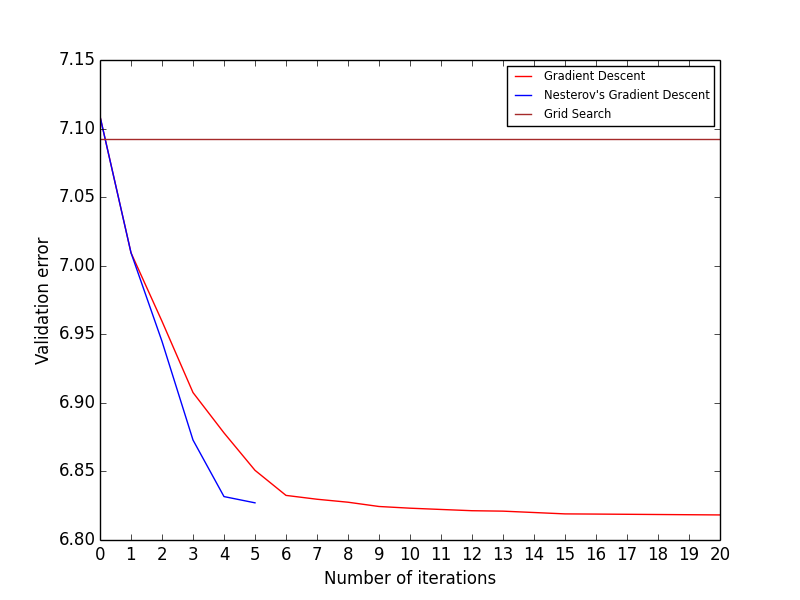
\includegraphics[width=70mm]{elasticnet_costpath_80_250_15.png}
%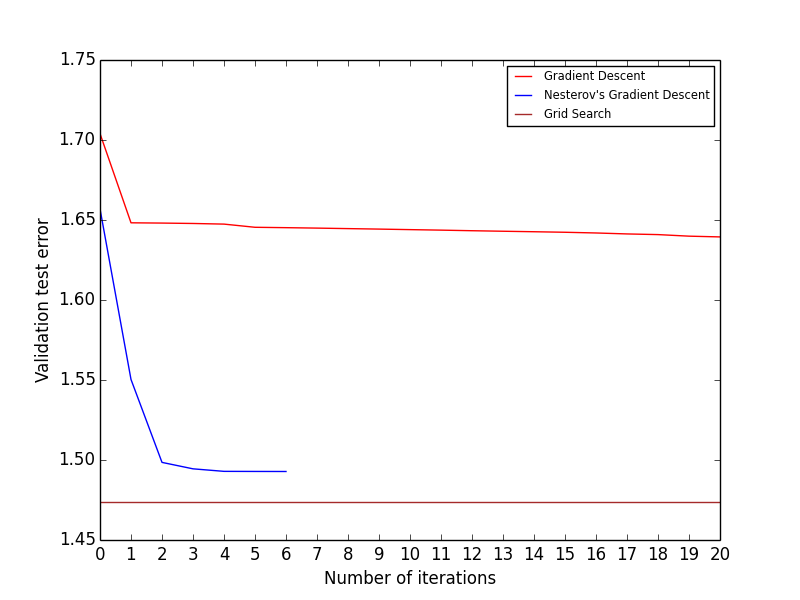
\includegraphics[width=70mm]{grouped_lasso_60_1500_3_150.png}
%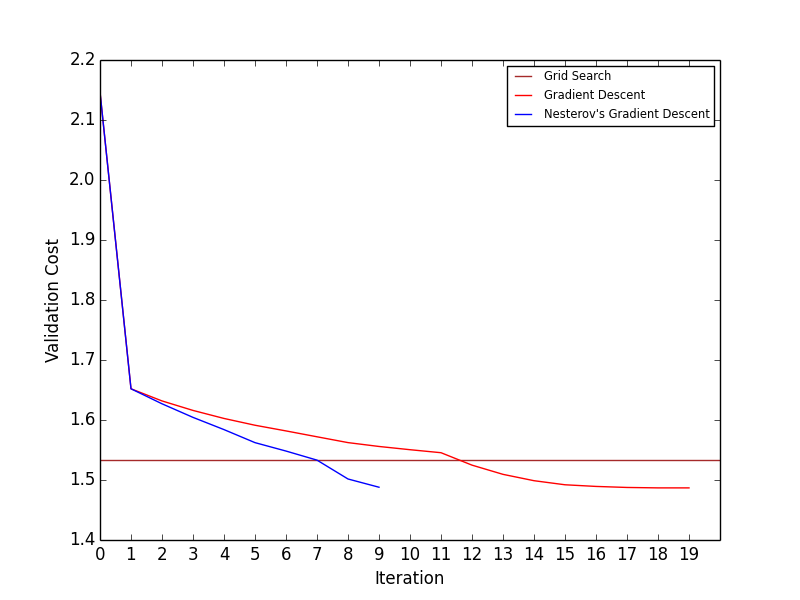
\includegraphics[width=70mm]{smooth_linear_simple_cost_path_1_100_20_6.png}
%\caption{Validation error progression: Top Left - Elastic Net, Top Right - Grouped Lasso, Bottom Left - APLM. \textcolor{red}{I know I asked for these... but I'm not sure if they are useful =]}}
%\label{figure:costpath}
%\end{figure}

\subsection{Discussion of results}

As shown in Table \ref{table:validation}, the descent-based and grid-based joint optimization have the same average performance in all three regression examples. Therefore, for simple regularization methods where the two methods are directly comparable, we see that they have the same performance.

We also note that descent-based joint optimization is faster than grid-based optimization in this setting, though not significantly so. For regularization methods with one or two penalty parameters, we don't expect huge efficiency gains from descent-based joint optimization.

\section{Results: regularizations with more than two penalties}

In this second simulation study, we test descent-based joint optimization on regressions with more than two regularization parameters. We are interested in whether descent-based joint optimization can find better model fits and also run efficiently.

We experiment with generalizations of the simple regressions from the previous section. That is, for the sparse group lasso, we made an ``unpooled" version in which the number of regularization parameters is one plus the number of covariate groups. For the APLM example, we added ridge penalty as a third regularization term. Details regarding the joint optimization problem formulations and gradient derivations for these generalized regression models are located in the Appendix.

We used gradient descent to tune the parameters for these more complex regularization methods. For baseline comparison, we also tuned the parameters for the original two-parameter regressions. Finally, we compared the accuracy of the models on a separate test set. The results show that gradient descent produced model fits for the generalized regressions that achieved lower test error. In addition, it remained computationally tractable, even in cases with over a hundred regularization parameters.

\subsection{Unpooled sparse group lasso}

In unpooled sparse group lasso, the group lasso penalty parameter $\lambda_1$ is replaced with an individual parameter for each covariate group

\begin{equation}
\sum_{j=1}^m \lambda_1^{(j)} \lvert\lvert \beta^{(j)} \rvert \rvert_2
+ \lambda_2 \lvert\lvert \beta \rvert \rvert_1
\label{unpooledSGL}
\end{equation}
The number of regularization parameters in \eqref{unpooledSGL} is then one plus the number of coefficient groups. This generalized criterion gives models the additional flexibility of having different thresholds for setting covariate and covariate group effects to zero. Therefore, unpooled sparse group lasso can potentially better model covariate groups with very different distributions.

We ran three experiments with different numbers of covariate groups $m$ and total covariates $p$, as given in Table \ref{table:unpooled}. The simulation settings were similar to the previous sparse group lasso simulation study. We used the same grid for grid-based joint optimization. For gradient descent, the $m+1$ regularization parameters were initialized at $1e\text{-}4 \times \boldsymbol 1^\top$, $1e\text{-}3 \times \boldsymbol 1^\top$, and $1e\text{-}2 \times \boldsymbol 1^\top$.

We measured three metrics to assess model performance: test error, $\beta$ error, which is defined as $\lvert \lvert \beta - \hat \beta \rvert \rvert_2 ^2$, and the percentage of nonzero coefficients correctly identified among all the true nonzero coefficients. The results show that unpooled sparse group lasso tuned using gradient descent performed better by all three metrics. Furthermore, gradient descent was significantly faster in all settings. The runtimes show that gradient descent does not grow with the number of regularization parameters.

\begin{table}
\begin{center}
\begin{tabular}{| l | l | l | l | l | }
\hline
\multicolumn{5}{|c|}{n=60, p=300, g=3, m=30}\\
\hline
 & $\beta$ Error & \% correct nonzero $\beta$ & Test Error & Runtime (sec) \\
\hline
Gridsearch (baseline) & 1.13 & 10.70 & 0.04 & 15.81 \\
\hline
Gradient Descent & 0.18 & 23.79 & 0.01 & 5.62 \\
\hline
\end{tabular}

%\vspace{5mm}
\begin{tabular}{| l | l | l | l | l | }
\hline
\multicolumn{5}{|c|}{n=60, p=1500, g=3, m=50}\\
\hline
 & $\beta$ Error & \% correct nonzero $\beta$ & Test Error & Runtime (sec) \\
\hline
Gridsearch (baseline) & 7.79 & 9.63 & 0.28 & 148.64 \\
\hline
Gradient Descent & 4.00 & 17.79 & 0.14 & 88.78 \\
\hline
\end{tabular}

%\vspace{5mm}
\begin{tabular}{| l | l | l | l | l | }
\hline
\multicolumn{5}{|c|}{n=60, p=1500, g=3, m=150}\\
\hline
 & $\beta$ Error & \% correct nonzero $\beta$ & Test Error & Runtime (sec) \\
\hline
Gridsearch (baseline) & 2.20 & 10.69 & 0.080 & 162.14 \\
\hline
Gradient Descent & 0.06 & 15.34 & 0.002 & 48.63 \\
\hline
\end{tabular}
\end{center}
\caption {Unpooled sparse group lasso}
\label{table:unpooled}
\end{table}

\subsection{Additive partial linear models with three regularization parameters}
We generalized the APLM criterion in \eqref{aplmProblem} by using the elastic net instead of the lasso:
\begin{equation}
\lambda_1 \lvert\lvert \beta \rvert \rvert_1
+ \frac{1}{2} \lambda_2 \lvert\lvert \beta \rvert \rvert_2^2
+ \frac{1}{2} \lambda_3 \lvert\lvert D^{(2)} \theta \rvert \rvert_2^2
\end{equation}
In the simulation, we tested the hypothesis that having the elastic net could better model data with sparse effects and strongly correlated predictors.

We ran experiments on three nonlinear functions of varying levels of smoothness as given in Table \ref{ref:aplm}. The simulation settings were similar to before. The only difference was that gradient descent was initialized at $10^i \times \boldsymbol 1^\top$ for $i=-4, ..., 1$.

Models were judged by their accuracy on the test set. In addition, we measured the error in the fitted linear model and nonparametric estimates with $\beta$ error=$||\beta - \hat \beta||_2^2$ and $\theta$ error=$|| g(z) - \theta ||_2^2$, respectively.

The results show that this generalized APLM criterion was better by all three metrics. The linear model fits improved the most, which is expected since the generalized model added a penalty to the linear coefficients. Surprisingly, the estimation of the nonlinear components also improved slightly, even though no penalty term was added for the nonparametric estimates. The runtime for tuning the three-parameter regularization was slightly longer than tuning two parameters with the grid-based method. Nonetheless, the runtime remained reasonable.

%In Figure \ref{fig:modelfits}, we show example model fits from gradient descent and grid-based joint optimization. The plots confirm the hypothesis that the highly-correlated covariates are estimated better using the three-parameter regularization as opposed to the two-parameter one.


\begin{table}
\begin{center}
\begin{tabular}{| l | l | l | l | l | }
\hline
\multicolumn{5}{|c|}{$g(z) = 4z^3 - z^2 + 2z$}\\
\hline
 & $\beta$ Error & $\theta$ error & Test Error & Runtime (sec) \\
\hline
Gridsearch & 0.59 & 3.35 & 3.78 & 35.48 \\
\hline
Gradient Descent & 0.38 & 2.96 & 3.73 & 43.44 \\
\hline
\end{tabular}

%\vspace{5mm}
\begin{tabular}{| l | l | l | l | l | }
\hline
\multicolumn{5}{|c|}{$g(z) = \sin(5z) + \sin(15(z - 3))$}\\
\hline
 & $\beta$ Error & $\theta$ error & Test Error & Runtime (sec) \\
\hline
Gridsearch & 0.51 & 3.76 & 3.90 & 37.04 \\
\hline
Gradient Descent & 0.34 & 3.73 & 3.79 & 45.95 \\
\hline
\end{tabular}

%\vspace{5mm}
\begin{tabular}{| l | l | l | l | l | }
\hline
\multicolumn{5}{|c|}{$g(z) = (2-z)\sin(20z^4)$}\\
\hline
 & $\beta$ Error & $\theta$ error & Test Error & Runtime (sec) \\
\hline
Gridsearch & 0.58 & 4.91 & 4.13 & 40.75 \\
\hline
Gradient Descent & 0.41 & 4.85 & 4.08 & 54.63 \\
\hline
\end{tabular}
\end{center}
\caption {Additive Partial Linear Model}
\label{ref:aplm}
\end{table}

%\begin{figure}
%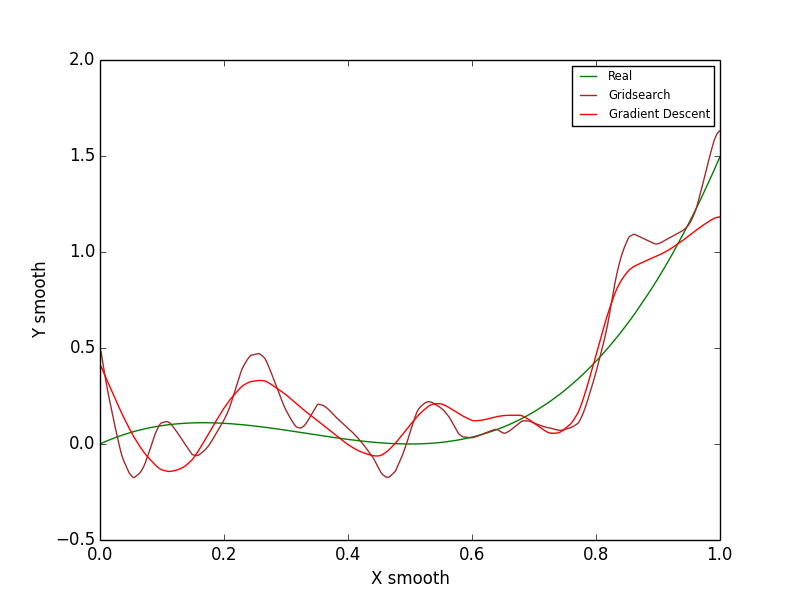
\includegraphics[height=40mm]{smooth_linear_thetas_2_100_20_6.png}
%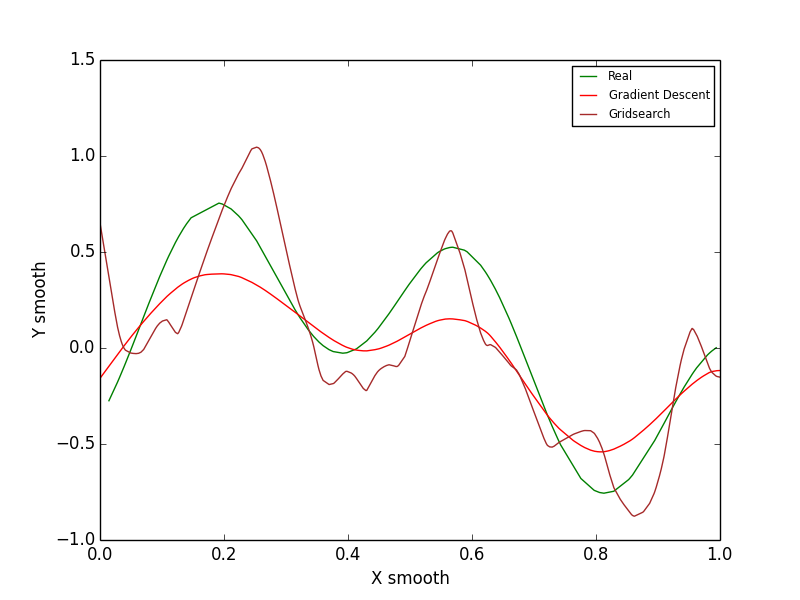
\includegraphics[height=40mm]{smooth_linear_thetas_0_100_20_6.png}
%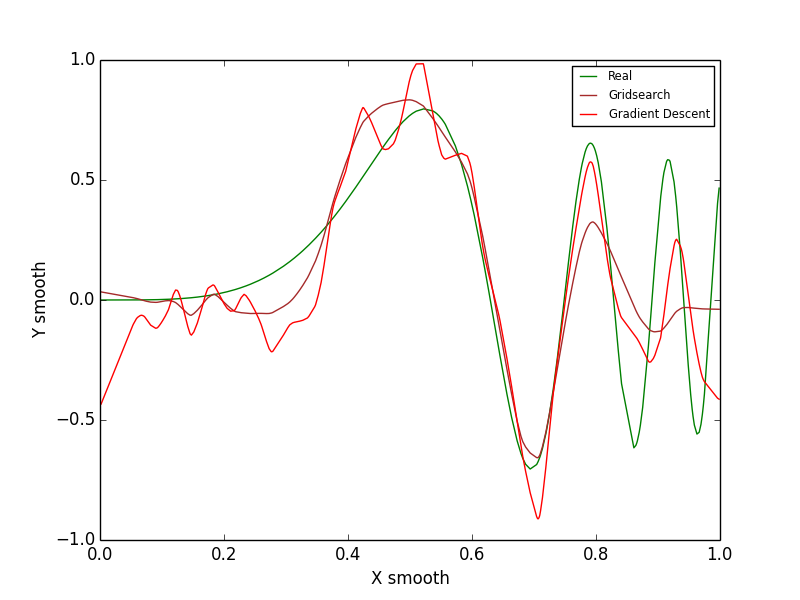
\includegraphics[height=40mm]{smooth_linear_thetas_1_100_20_6.png}
%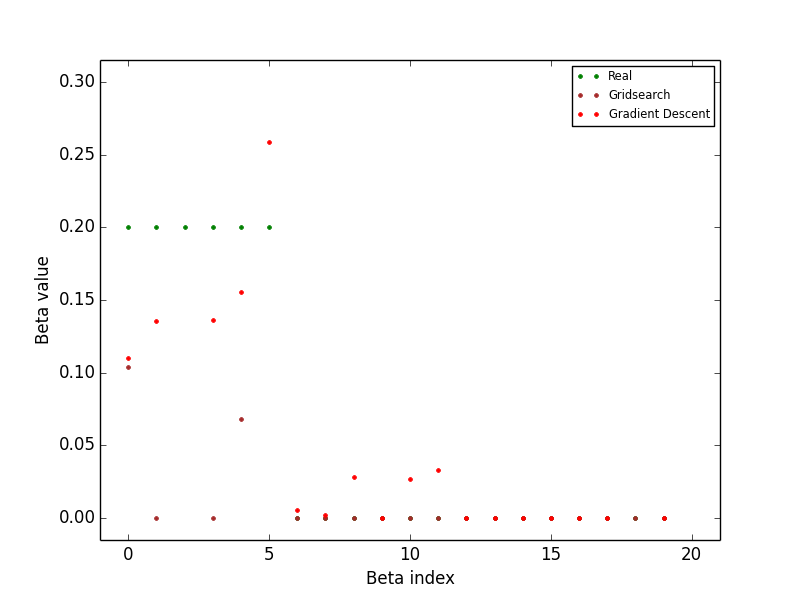
\includegraphics[height=40mm]{smooth_linear_beta_2_100_20_6.png}
%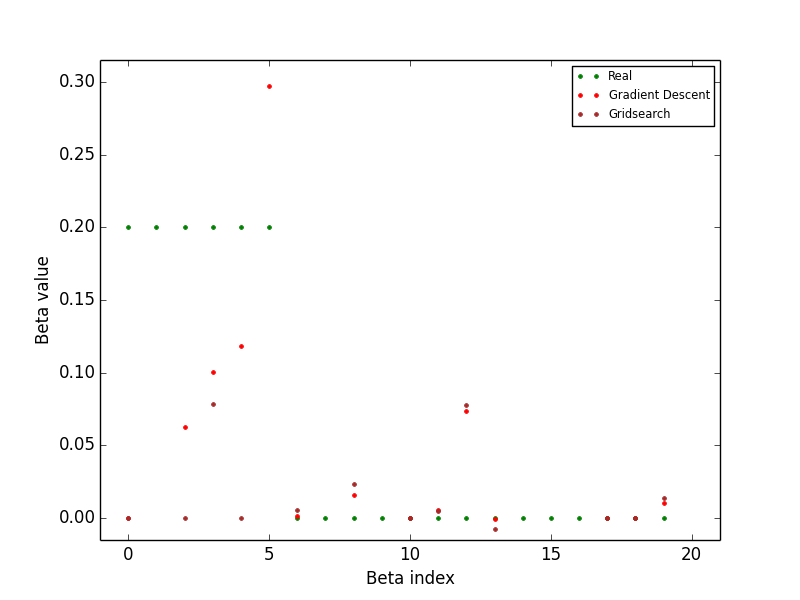
\includegraphics[height=40mm]{smooth_linear_beta_0_100_20_6.png}
%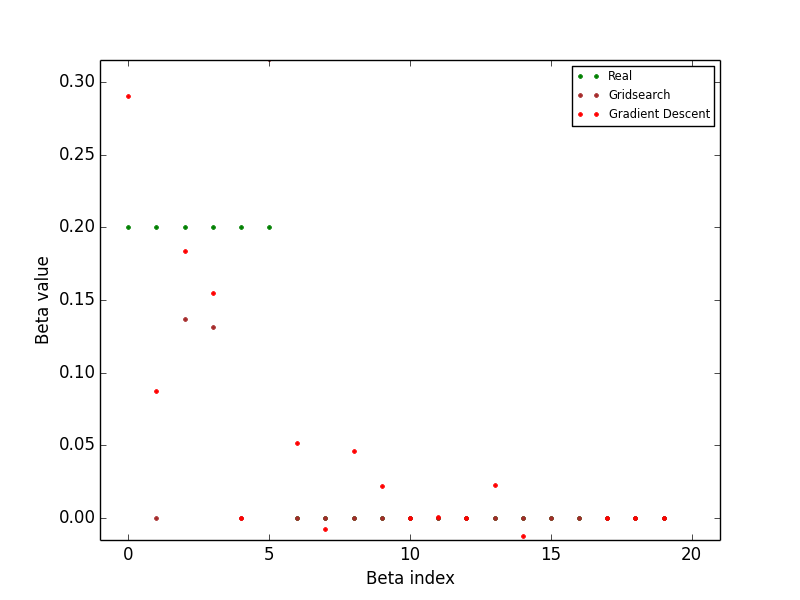
\includegraphics[height=40mm]{smooth_linear_beta_1_100_20_6.png}
%\caption{Top: Example fits to the three smooth functions used in the experiments. The green line is the true function. Bottom: Example fits for the linear regression coefficients. The green is the true beta. \textcolor{red}{I know I asked for these... but I'm not sure if they are useful =]}}
%\label{fig:modelfits}
%\end{figure}

\section{Application to Real Data}
In this section, we apply descent-based joint optimization to real data.

We apply un-pooled sparse group lasso to the real-data application from \citet{simon2013sparse}. For comparison, we also fit the sparse group lasso model. In this problem, we are interested in finding genes from gene pathways that are driving Crohn's Disease and Ulcerative Colitis.

Our dataset is from a colitis study of 127 total patients, 85 with colitis (59 crohn's patients + 26 ulcerative colitis patients) and 42 health controls \citep{burczynski2006molecular}. Expression data was measured for 22,283 genes on affymetrix U133A microarrays. We grouped the genes according to the 326 C1 positional gene sets from MSigDb v5.0 \citep{subramanian2005gene} and discarded the 2358 genes not found in the gene set.

For each experiment, we randomly shuffled the data and used the first 50 observations for the training set and the remaining 77 for the test set. The experiment was repeated 10 times. 5-fold cross-validation was used to fit models. The penalty parameters in un-pooled sparse group lasso were initialized at $0.5 \times \boldsymbol 1^\top$. For sparse group lasso, models were fit over a $5 \times 5$ grid of parameter values from 1e-4 to 5.

As shown in Table \ref{colitis}, un-pooled sparse group lasso achieved a slightly higher classification rate compared to sparse group lasso. Interestingly, un-pooled sparse group lasso finds solutions that are significantly more sparse than sparse group lasso -- on average, 9 genesets were identified, as opposed to 38. In addition, the number of genesets identified by un-pooled sparse group lasso has significantly lower variance. The number of genesets identified by sparse group lasso ranged from 2 to 73, whereas the number of genesets identified by un-pooled sparse group lasso ranged from 8 to 12. These results suggest that un-pooling the penalty parameters in sparse group lasso could potentially improve interpretability and stability.

Perhaps the most significant result from this section is the fact that fitting the un-pooled sparse group lasso with 327 regularization parameters is computationally tractable. Its runtime was slightly lower than sparse group lasso even though the latter only has two regularization parameters.

\begin{table}
\begin{center}
\begin{tabular}{| l | l | l | l | l | }
\hline
 & \% correct  & Num. Genesets & Num. Genes & Runtime (sec) \\
\hline
SGL & 82.47 (0.7) & 38.4 (671.2) & 207.0 (22206.2) & 2722.4 \\
\hline
Unpooled SGL & 84.29 (0.3) & 8.9 (1.9) & 83.9 (664.5) & 2298.5 \\
\hline
\end{tabular}
\end{center}
\caption {Ulcerative Colitis Data: SGL = sparse group lasso, variance in parentheses}
\label{colitis}
\end{table}

\section{Discussion}
In this paper, we proposed finding the optimal regularization parameters by treating it as an optimization problem over the regularization parameter space. We have proven that a descent-based approach can be used for regression problems in which the penalties are smooth almost everywhere and present a general algorithm for performing a modified gradient descent.

Empirically, we find that models fit by descent-based joint optimization have similar accuracy to those from grid-based methods. Furthermore, the scalability of this approach allows us to test new regularization methods with many regularization parameters. In particular, we found that an un-pooled variant of sparse group lasso showed promising results. Further research should be done to explore this new regularization method.

Future work could include finding other classes of regularization methods that are suitable for descent-based joint optimization and implementing descent-based joint optimization with more sophisticated optimization methods.

\section{Appendix}

\subsection{Proof of Theorem \ref{thethrm}}

\begin{proof}
It is sufficient to show that the theorem holds for a given $\lambda_0$. For a given $\lambda_0$, let $B'$ be the basis vectors that span the differentiable space $\Omega^{L_T}(\hat \theta(\lambda_0), \lambda_0)$. Let $B$ be the subset of the basis vectors that span the model parameter space.

Let $\tilde L_T(\theta, \lambda)$ be the gradient of $L_T(\cdot, \lambda)$ at $\theta$ with respect to the basis $B$:
\begin{equation}
\tilde L(\theta, \lambda) = \nabla_{B} L_T(\cdot, \lambda) |_\theta
\end{equation}

Since $\hat \theta(\lambda_0)$ is the minimizer of the training loss, the gradient of $L_T(\cdot, \lambda_0)$ with respect to the basis $B$ must be zero at $\hat \theta(\lambda_0)$:
\begin{equation}
\nabla_{B} L_T(\cdot, \lambda_0)|_{\hat \theta(\lambda_0)} = \tilde L_T(\hat \theta(\lambda_0), \lambda_0) = 0
\end{equation}

From our assumptions, we know that there exists a neighborhood $W$ such that $\tilde L_T$ is continuously differentiable along directions in the differentiable space $\Omega^{L_T}(\hat \theta(\lambda_0), \lambda_0)$. Also, the Jacobian matrix $D \tilde L_T(\cdot, \lambda_0)|_{\hat \theta(\lambda_0)}$ with respect to basis $B$ is nonsingular. Therefore, by the implicit function theorem, there exist open sets $U$ containing $\lambda_0$ and $V$ containing $\hat \theta(\lambda_0)$ and a continuously differentiable function $\gamma: U \rightarrow V$ such that for every $\lambda \in U$, we have that 
\begin{equation}
\tilde L_T(\gamma(\lambda), \lambda) = \nabla_{B} L_T(\cdot, \lambda)|_{\gamma(\lambda)} = 0
\end{equation}
That is, we know that $\gamma(\lambda)$ is a continuously differentiable function that minimizes $L_T(\cdot, \lambda)$ in the differentiable space  $\Omega^{L_T}(\hat \theta(\lambda_0), \lambda_0)$.
Since we assumed that the differentiable space is a local optimality space of $L_T(\cdot, \lambda)$ in the neighborhood $W$, then there must exist some neighborhood $W'$ containing $\lambda_0$ such that for every $\lambda \in W'$, 
\begin{equation}
\hat \theta(\lambda) =
\argmin_\theta L_T(\theta, \lambda) =
\argmin_{\theta \in \Omega^{L_T}(\hat \theta(\lambda_0), \lambda_0)} L_T(\theta, \lambda) =
\gamma(\lambda)
\end{equation}
Therefore, we have shown that if $\lambda_0$ satisfies the assumptions given in the theorem, the fitted model parameters $\hat \theta(\lambda)$ is a continuously differentiable function within a neighborhood of $\lambda_0$. If the assumptions in the theorem hold true for almost every set of regularization parameters, then $\hat \theta(\lambda)$ is continuously differentiable almost everywhere. Furthermore, the Jacobian matrix of the model parameters, where it is defined, is
\begin{equation}
\frac{\partial}{\partial \lambda} \hat \theta(\lambda) = \frac{\partial}{\partial \lambda} \dot \theta(\lambda)
\end{equation}
where 
\begin{equation}
\dot \theta(\lambda) = \argmin_{\theta \in \Omega^{L_T}(\hat \theta(\lambda_0), \lambda_0)} L_T(\theta, \lambda)
\end{equation}
We can then apply the chain rule to get the gradient of the validation loss.
\end{proof}

%\begin{lemma}
%Given a real-valued function $L(f, \lambda)$ and some point $\lambda_0$, let
%\begin{equation}
%\Omega^{(\lambda_0)} = \text{span}(\{\delta | \lim_{\epsilon \rightarrow 0} \frac{L(f + \epsilon \delta, \lambda) - L(f, \lambda)}{\epsilon} \text{ exists} \})
%\end{equation}
%and suppose there exists some neighborhood $B$ around $\lambda_0$ such that for every $\lambda \in B$, $\text{proj}_{\Omega_{\bot}^{(\lambda_0)}} \hat f(\lambda)=0$. Then for every $\lambda \in B$,
%\begin{equation}
%\hat f(\lambda) = \argmin_{f' \in \Omega^{(\lambda_0)}} L(f', \lambda)
%\end{equation}
%\label{lemma2}
%\end{lemma}
%
%\begin{proof}
%From the assumption, we have that
%\begin{equation}
%\hat f(\lambda) = \text{proj}_{\Omega_{\bot}^{(\lambda_0)}} \hat f(\lambda) + \text{proj}_{\Omega^{(\lambda_0)}} \hat f(\lambda) = \text{proj}_{\Omega^{(\lambda_0)}} \hat f(\lambda)
%\end{equation}
%which implies that minimizing $L(f, \lambda)$ over the subspace $\Omega^{(\lambda_0)}$ is equivalent to minimizing over the entire space.
%\end{proof}


%\begin{lemma}
%Let $\hat f(\cdot)$ be defined as in lemma 1. For a given $\lambda_0$, suppose there exists a neighborhood around $f(\lambda_0)$ such that the regularity conditions from lemma 1 for $L(f, \lambda_0)$ only hold with respect to the active set of $f$. Furthermore, suppose there exists a neighborhood around $\lambda_0$ such that the non-active set of $\hat f(\cdot)$ is locally constant. Then $\hat f(\cdot)$ is continuously differentiable in some neighborhood around $\lambda_0$.
%\label{activesetthrm}
%\end{lemma}
%
%\begin{proof}
%By the KKT conditions, $\hat f(\lambda_0)$ is the point where the following subgradient condition is satisfied:
%
%\begin{equation}
%0 \in \partial_f L(f, \lambda_0)
%\end{equation}
%
%For the active set $\dot f$, the subgradient condition reduces to the gradient condition:
%
%\begin{equation}
%0 = \nabla_{\dot f} L(f, \lambda_0)
%\label{gradientcondition}
%\end{equation}
%
%Applying Theorem \ref{differentiablethrm} to the gradient condition in (\ref{gradientcondition}), we know that the active set $\dot f(\cdot)$ is continuously differentiable for some neighborhood around $\lambda_0$. By our assumptions, the partial derivative of $\hat f(\cdot)$ with respect to the non-active set is zero in some neighborhood around $\lambda_0$. Combining the active and non-active sets, we have that $\hat f(\cdot)$ is continuously differentiable in some neighborhood around $\lambda_0$.
%
%\end{proof}

\subsection{Gradient Derivations}

\subsubsection{Unpooled 
}
The gradient of the validation error with respect to the regularization parameters is:
\begin{equation}
\begin{array}{lcl}
\nabla_{\lambda_1^{(k)}} L(\boldsymbol y_V, X_V \hat \beta) &=& 
\frac{1}{n}
\Bigg (
X_V
(\frac{1}{n} X^\top X + M_1 + M_2)^{-1}
\begin{bmatrix}
0 \\
\vdots \\
\frac{\hat\beta^{(l}}{||\hat\beta^{(l}||_2}\\
\vdots\\
0
\end{bmatrix}
\Bigg )^\top
(\boldsymbol y_V - X_V \hat \beta)
 \\
\nabla_{\lambda_2} L(\boldsymbol y_V, X_V \hat \beta) &=&
\frac{1}{n}
\Bigg (
(\frac{1}{n} X^\top X + M_1 + M_2)^{-1} sign(\hat \beta)
\Bigg )^\top
(\boldsymbol y_V - X_V \hat \beta)
\\ 
\end{array}
\end{equation}

where $M_1$ is the block diagonal matrix with $l$ components 
$
\frac{\lambda_1^{(k)}}{|| \beta^{(k)}||_2^3}
\begin{bmatrix} 
\beta_1^{(k)} & 0 & \\
0 & \beta_2^{(k)} &  \\
 &  & \ddots \\
\end{bmatrix}
\begin{bmatrix}
\text{---} & \beta^{(k)T} & \text{---} \\
\text{---} & \beta^{(k)T} & \text{---} \\
\vdots
\end{bmatrix}
$ from top left to bottom right and $M_2$ is the diagonal matrix with $\frac{\lambda_1^{(k)}}{|| \beta^{(k)}||_2}$ from top left to bottom right.

\subsubsection{Additive Partial Linear Model with three penalties}

To perform joint optimization, we formulate the problem as follows:
\begin{multline}
\min_{\lambda_1, \lambda_2, \lambda_3} \frac{1}{2} \bigl\lvert\bigl\lvert \boldsymbol y_V - X_V\hat\beta - M_V \hat\theta \bigl\rvert\bigl\rvert^2_2 \\
\text{ where } \hat\beta, \hat\theta = \argmin_{\beta, \theta} \frac{1}{2} \bigl\lvert\bigl\lvert y - X\beta - M_T \theta \bigl\rvert\bigl\rvert^2_2
+ \lambda_1 \lvert\lvert \beta \rvert \rvert_1
+ \frac{1}{2} \lambda_2 \lvert\lvert \beta \rvert \rvert_2^2
+ \frac{1}{2} \lambda_3 \lvert\lvert D^{(2)} \theta \rvert \rvert_2^2
\end{multline}
where $M_V \in \mathbb{R}^{|V| \times n}$ is the matrix such that $M_V X = X_V$ and $M_T \in \mathbb{R}^{|T| \times n}$ is the matrix such that $M_T X = X_T$ .

The gradients of the validation set error with respect to the regularization parameters are:
\begin{equation}
\nabla_{\lambda_i} L(\boldsymbol y_V, X_V \hat \beta + \hat \theta) = (X_V \frac{\partial \beta}{\partial \lambda_i} + M_V \frac{\partial \theta}{\partial \lambda_i})^\top(\boldsymbol y_V - X_V \hat \beta - \hat \theta_V)
\end{equation}
where
\begin{equation}
\begin{array}{lcl}
\frac{\partial \beta}{\partial \lambda_1} &=& -(X_T^\top X_T - X_T^\top M_T(M_T^\top M_T + \lambda_3 D^\top D)^{-1} M_T^\top X_T + \lambda_2 I)^{-1} sign(\hat \beta) \\
\frac{\partial \theta}{\partial \lambda_1} &=& -(M_T^\top M_T + \lambda_3 D^\top D)^{-1}  M_T^\top X_T \frac{\partial \beta}{\partial \lambda_1}
\\
\frac{\partial \beta}{\partial \lambda_2} &=& -(X_T^\top X_T - X_T^\top M_T(M_T^\top M_T + \lambda_3 D^\top D)^{-1} M_T^\top X_T + \lambda_2 I)^{-1} \hat \beta \\
\frac{\partial \theta}{\partial \lambda_2} &=& -(M_T^\top M_T + \lambda_3 D^\top D)^{-1}  M_T^\top X_T \frac{\partial \beta}{\partial \lambda_2}
\\
\frac{\partial \theta}{\partial \lambda_3} &=& -(M_T^\top M_T - M_T^\top X_T (X_T^\top X_T + \lambda_2 I)^{-1} X_T^\top M_T + \lambda_3 D^\top D)^{-1} D^\top D \theta
\\
\frac{\partial \beta}{\partial \lambda_3} &=& - (X_T^\top X_T + \lambda_2 I)^{-1} X_T^\top M_T \frac{\partial \theta}{\partial \lambda_3} \\
\end{array}
\end{equation}

\section*{Acknowledgments}


\bibliographystyle{abbrvnat}
\bibliography{hillclimbing}
% Command: pdflatex hillclimbing.tex; bibtex hillclimbing; pdflatex hillclimbing.tex
\end{document}

